% Created by tikzDevice version 0.12.3.1 on 2021-02-24 21:50:54
% !TEX encoding = UTF-8 Unicode
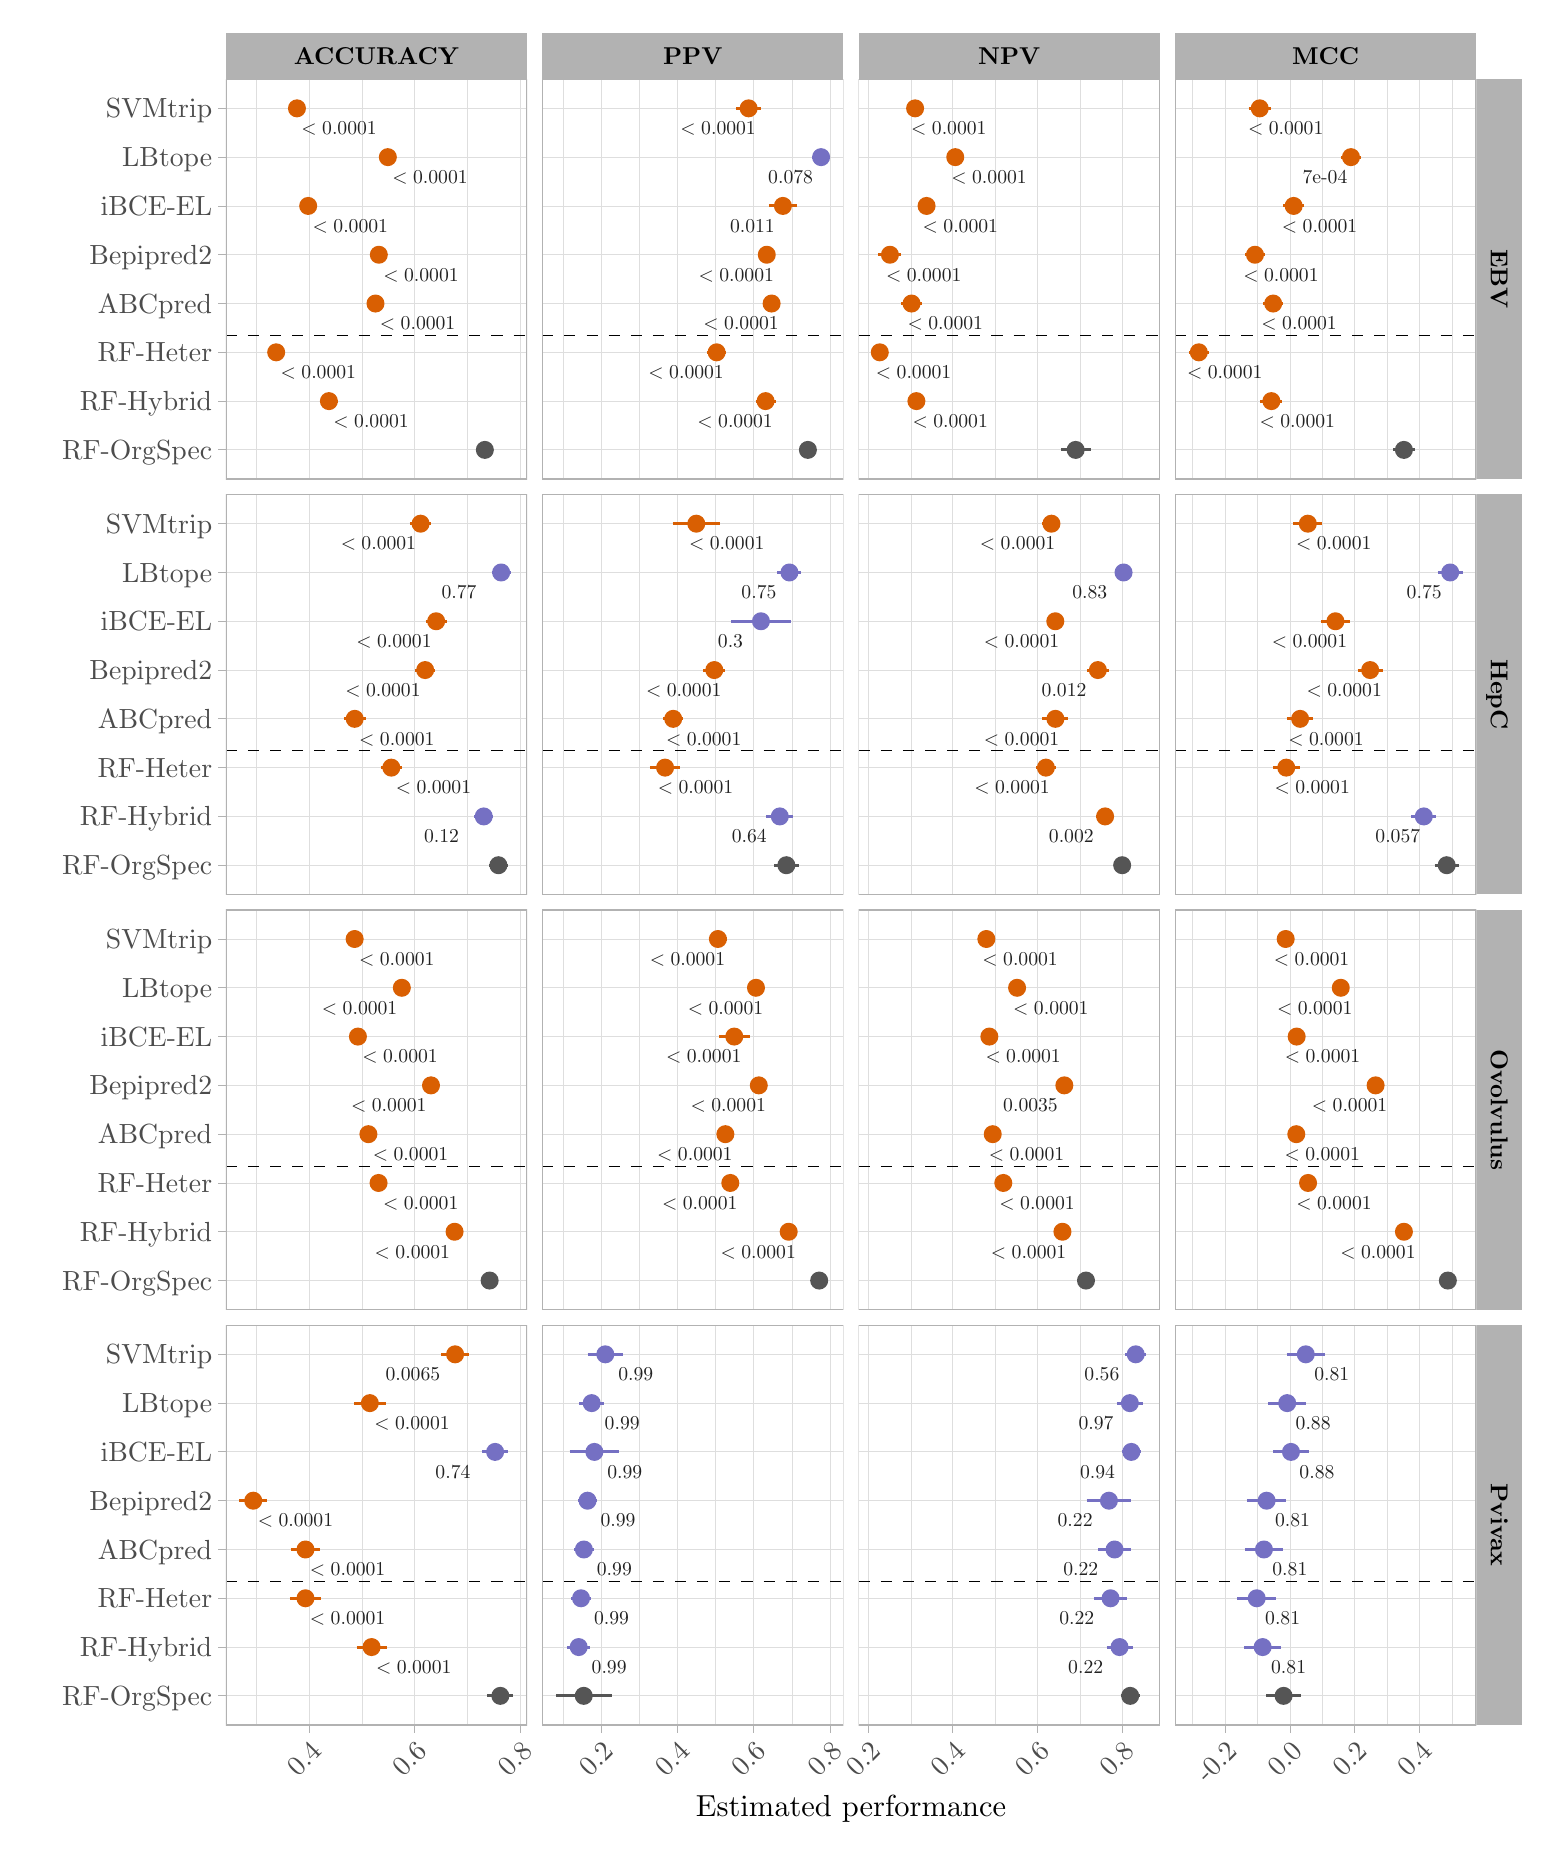
\begin{tikzpicture}[x=1pt,y=1pt]
\definecolor{fillColor}{RGB}{255,255,255}
\path[use as bounding box,fill=fillColor,fill opacity=0.00] (0,0) rectangle (542.02,650.43);
\begin{scope}
\path[clip] (  0.00,  0.00) rectangle (542.02,650.43);
\definecolor{drawColor}{RGB}{255,255,255}
\definecolor{fillColor}{RGB}{255,255,255}

\path[draw=drawColor,line width= 0.6pt,line join=round,line cap=round,fill=fillColor] ( -0.00,  0.00) rectangle (542.02,650.43);
\end{scope}
\begin{scope}
\path[clip] ( 71.60,487.27) rectangle (180.43,631.85);
\definecolor{fillColor}{RGB}{255,255,255}

\path[fill=fillColor] ( 71.60,487.27) rectangle (180.43,631.85);
\definecolor{drawColor}{gray}{0.87}

\path[draw=drawColor,line width= 0.1pt,line join=round] ( 82.71,487.27) --
	( 82.71,631.85);

\path[draw=drawColor,line width= 0.1pt,line join=round] (120.81,487.27) --
	(120.81,631.85);

\path[draw=drawColor,line width= 0.1pt,line join=round] (158.92,487.27) --
	(158.92,631.85);

\path[draw=drawColor,line width= 0.3pt,line join=round] ( 71.60,497.85) --
	(180.43,497.85);

\path[draw=drawColor,line width= 0.3pt,line join=round] ( 71.60,515.48) --
	(180.43,515.48);

\path[draw=drawColor,line width= 0.3pt,line join=round] ( 71.60,533.11) --
	(180.43,533.11);

\path[draw=drawColor,line width= 0.3pt,line join=round] ( 71.60,550.74) --
	(180.43,550.74);

\path[draw=drawColor,line width= 0.3pt,line join=round] ( 71.60,568.37) --
	(180.43,568.37);

\path[draw=drawColor,line width= 0.3pt,line join=round] ( 71.60,586.01) --
	(180.43,586.01);

\path[draw=drawColor,line width= 0.3pt,line join=round] ( 71.60,603.64) --
	(180.43,603.64);

\path[draw=drawColor,line width= 0.3pt,line join=round] ( 71.60,621.27) --
	(180.43,621.27);

\path[draw=drawColor,line width= 0.3pt,line join=round] (101.76,487.27) --
	(101.76,631.85);

\path[draw=drawColor,line width= 0.3pt,line join=round] (139.86,487.27) --
	(139.86,631.85);

\path[draw=drawColor,line width= 0.3pt,line join=round] (177.97,487.27) --
	(177.97,631.85);
\definecolor{drawColor}{RGB}{85,85,85}

\path[draw=drawColor,line width= 1.1pt,line join=round] (162.34,497.85) -- (168.05,497.85);
\definecolor{drawColor}{RGB}{217,95,2}

\path[draw=drawColor,line width= 1.1pt,line join=round] (105.72,515.48) -- (111.99,515.48);

\path[draw=drawColor,line width= 1.1pt,line join=round] ( 86.97,533.11) -- ( 92.63,533.11);

\path[draw=drawColor,line width= 1.1pt,line join=round] (122.72,550.74) -- (128.64,550.74);

\path[draw=drawColor,line width= 1.1pt,line join=round] (123.79,568.37) -- (129.99,568.37);

\path[draw=drawColor,line width= 1.1pt,line join=round] ( 98.25,586.01) -- (104.46,586.01);

\path[draw=drawColor,line width= 1.1pt,line join=round] (127.06,603.64) -- (133.21,603.64);

\path[draw=drawColor,line width= 1.1pt,line join=round] ( 94.21,621.27) -- (100.39,621.27);
\definecolor{drawColor}{RGB}{85,85,85}
\definecolor{fillColor}{RGB}{85,85,85}

\path[draw=drawColor,line width= 0.8pt,line join=round,line cap=round,fill=fillColor] (165.20,497.85) circle (  2.85);
\definecolor{drawColor}{RGB}{217,95,2}
\definecolor{fillColor}{RGB}{217,95,2}

\path[draw=drawColor,line width= 0.8pt,line join=round,line cap=round,fill=fillColor] (108.85,515.48) circle (  2.85);

\path[draw=drawColor,line width= 0.8pt,line join=round,line cap=round,fill=fillColor] ( 89.80,533.11) circle (  2.85);

\path[draw=drawColor,line width= 0.8pt,line join=round,line cap=round,fill=fillColor] (125.68,550.74) circle (  2.85);

\path[draw=drawColor,line width= 0.8pt,line join=round,line cap=round,fill=fillColor] (126.89,568.37) circle (  2.85);

\path[draw=drawColor,line width= 0.8pt,line join=round,line cap=round,fill=fillColor] (101.36,586.01) circle (  2.85);

\path[draw=drawColor,line width= 0.8pt,line join=round,line cap=round,fill=fillColor] (130.14,603.64) circle (  2.85);

\path[draw=drawColor,line width= 0.8pt,line join=round,line cap=round,fill=fillColor] ( 97.30,621.27) circle (  2.85);
\definecolor{drawColor}{RGB}{34,34,34}

\node[text=drawColor,anchor=base,inner sep=0pt, outer sep=0pt, scale=  0.71] at (124.10,505.98) {$<0.0001$};

\node[text=drawColor,anchor=base,inner sep=0pt, outer sep=0pt, scale=  0.71] at (105.04,523.61) {$<0.0001$};

\node[text=drawColor,anchor=base,inner sep=0pt, outer sep=0pt, scale=  0.71] at (140.92,541.24) {$<0.0001$};

\node[text=drawColor,anchor=base,inner sep=0pt, outer sep=0pt, scale=  0.71] at (142.13,558.87) {$<0.0001$};

\node[text=drawColor,anchor=base,inner sep=0pt, outer sep=0pt, scale=  0.71] at (116.60,576.50) {$<0.0001$};

\node[text=drawColor,anchor=base,inner sep=0pt, outer sep=0pt, scale=  0.71] at (145.38,594.13) {$<0.0001$};

\node[text=drawColor,anchor=base,inner sep=0pt, outer sep=0pt, scale=  0.71] at (112.54,611.77) {$<0.0001$};
\definecolor{drawColor}{RGB}{0,0,0}

\path[draw=drawColor,line width= 0.2pt,dash pattern=on 4pt off 4pt ,line join=round] ( 71.60,539.28) -- (180.43,539.28);
\definecolor{drawColor}{gray}{0.70}

\path[draw=drawColor,line width= 0.6pt,line join=round,line cap=round] ( 71.60,487.27) rectangle (180.43,631.85);
\end{scope}
\begin{scope}
\path[clip] ( 71.60,337.20) rectangle (180.43,481.77);
\definecolor{fillColor}{RGB}{255,255,255}

\path[fill=fillColor] ( 71.60,337.20) rectangle (180.43,481.77);
\definecolor{drawColor}{gray}{0.87}

\path[draw=drawColor,line width= 0.1pt,line join=round] ( 82.71,337.20) --
	( 82.71,481.77);

\path[draw=drawColor,line width= 0.1pt,line join=round] (120.81,337.20) --
	(120.81,481.77);

\path[draw=drawColor,line width= 0.1pt,line join=round] (158.92,337.20) --
	(158.92,481.77);

\path[draw=drawColor,line width= 0.3pt,line join=round] ( 71.60,347.78) --
	(180.43,347.78);

\path[draw=drawColor,line width= 0.3pt,line join=round] ( 71.60,365.41) --
	(180.43,365.41);

\path[draw=drawColor,line width= 0.3pt,line join=round] ( 71.60,383.04) --
	(180.43,383.04);

\path[draw=drawColor,line width= 0.3pt,line join=round] ( 71.60,400.67) --
	(180.43,400.67);

\path[draw=drawColor,line width= 0.3pt,line join=round] ( 71.60,418.30) --
	(180.43,418.30);

\path[draw=drawColor,line width= 0.3pt,line join=round] ( 71.60,435.93) --
	(180.43,435.93);

\path[draw=drawColor,line width= 0.3pt,line join=round] ( 71.60,453.56) --
	(180.43,453.56);

\path[draw=drawColor,line width= 0.3pt,line join=round] ( 71.60,471.19) --
	(180.43,471.19);

\path[draw=drawColor,line width= 0.3pt,line join=round] (101.76,337.20) --
	(101.76,481.77);

\path[draw=drawColor,line width= 0.3pt,line join=round] (139.86,337.20) --
	(139.86,481.77);

\path[draw=drawColor,line width= 0.3pt,line join=round] (177.97,337.20) --
	(177.97,481.77);
\definecolor{drawColor}{RGB}{85,85,85}

\path[draw=drawColor,line width= 1.1pt,line join=round] (166.74,347.78) -- (173.45,347.78);
\definecolor{drawColor}{RGB}{117,112,195}

\path[draw=drawColor,line width= 1.1pt,line join=round] (161.41,365.41) -- (168.19,365.41);
\definecolor{drawColor}{RGB}{217,95,2}

\path[draw=drawColor,line width= 1.1pt,line join=round] (127.50,383.04) -- (135.29,383.04);

\path[draw=drawColor,line width= 1.1pt,line join=round] (114.24,400.67) -- (122.09,400.67);

\path[draw=drawColor,line width= 1.1pt,line join=round] (139.92,418.30) -- (147.35,418.30);

\path[draw=drawColor,line width= 1.1pt,line join=round] (143.82,435.93) -- (151.39,435.93);
\definecolor{drawColor}{RGB}{117,112,195}

\path[draw=drawColor,line width= 1.1pt,line join=round] (167.66,453.56) -- (174.52,453.56);
\definecolor{drawColor}{RGB}{217,95,2}

\path[draw=drawColor,line width= 1.1pt,line join=round] (138.07,471.19) -- (145.90,471.19);
\definecolor{drawColor}{RGB}{85,85,85}
\definecolor{fillColor}{RGB}{85,85,85}

\path[draw=drawColor,line width= 0.8pt,line join=round,line cap=round,fill=fillColor] (170.10,347.78) circle (  2.85);
\definecolor{drawColor}{RGB}{117,112,195}
\definecolor{fillColor}{RGB}{117,112,195}

\path[draw=drawColor,line width= 0.8pt,line join=round,line cap=round,fill=fillColor] (164.80,365.41) circle (  2.85);
\definecolor{drawColor}{RGB}{217,95,2}
\definecolor{fillColor}{RGB}{217,95,2}

\path[draw=drawColor,line width= 0.8pt,line join=round,line cap=round,fill=fillColor] (131.40,383.04) circle (  2.85);

\path[draw=drawColor,line width= 0.8pt,line join=round,line cap=round,fill=fillColor] (118.17,400.67) circle (  2.85);

\path[draw=drawColor,line width= 0.8pt,line join=round,line cap=round,fill=fillColor] (143.63,418.30) circle (  2.85);

\path[draw=drawColor,line width= 0.8pt,line join=round,line cap=round,fill=fillColor] (147.60,435.93) circle (  2.85);
\definecolor{drawColor}{RGB}{117,112,195}
\definecolor{fillColor}{RGB}{117,112,195}

\path[draw=drawColor,line width= 0.8pt,line join=round,line cap=round,fill=fillColor] (171.09,453.56) circle (  2.85);
\definecolor{drawColor}{RGB}{217,95,2}
\definecolor{fillColor}{RGB}{217,95,2}

\path[draw=drawColor,line width= 0.8pt,line join=round,line cap=round,fill=fillColor] (141.98,471.19) circle (  2.85);
\definecolor{drawColor}{RGB}{34,34,34}

\node[text=drawColor,anchor=base,inner sep=0pt, outer sep=0pt, scale=  0.71] at (149.56,355.91) {0.12};

\node[text=drawColor,anchor=base,inner sep=0pt, outer sep=0pt, scale=  0.71] at (146.64,373.54) {$<0.0001$};

\node[text=drawColor,anchor=base,inner sep=0pt, outer sep=0pt, scale=  0.71] at (133.41,391.17) {$<0.0001$};

\node[text=drawColor,anchor=base,inner sep=0pt, outer sep=0pt, scale=  0.71] at (128.39,408.80) {$<0.0001$};

\node[text=drawColor,anchor=base,inner sep=0pt, outer sep=0pt, scale=  0.71] at (132.36,426.43) {$<0.0001$};

\node[text=drawColor,anchor=base,inner sep=0pt, outer sep=0pt, scale=  0.71] at (155.85,444.06) {0.77};

\node[text=drawColor,anchor=base,inner sep=0pt, outer sep=0pt, scale=  0.71] at (126.74,461.69) {$<0.0001$};
\definecolor{drawColor}{RGB}{0,0,0}

\path[draw=drawColor,line width= 0.2pt,dash pattern=on 4pt off 4pt ,line join=round] ( 71.60,389.21) -- (180.43,389.21);
\definecolor{drawColor}{gray}{0.70}

\path[draw=drawColor,line width= 0.6pt,line join=round,line cap=round] ( 71.60,337.20) rectangle (180.43,481.77);
\end{scope}
\begin{scope}
\path[clip] ( 71.60,187.12) rectangle (180.43,331.70);
\definecolor{fillColor}{RGB}{255,255,255}

\path[fill=fillColor] ( 71.60,187.12) rectangle (180.43,331.70);
\definecolor{drawColor}{gray}{0.87}

\path[draw=drawColor,line width= 0.1pt,line join=round] ( 82.71,187.12) --
	( 82.71,331.70);

\path[draw=drawColor,line width= 0.1pt,line join=round] (120.81,187.12) --
	(120.81,331.70);

\path[draw=drawColor,line width= 0.1pt,line join=round] (158.92,187.12) --
	(158.92,331.70);

\path[draw=drawColor,line width= 0.3pt,line join=round] ( 71.60,197.70) --
	(180.43,197.70);

\path[draw=drawColor,line width= 0.3pt,line join=round] ( 71.60,215.33) --
	(180.43,215.33);

\path[draw=drawColor,line width= 0.3pt,line join=round] ( 71.60,232.96) --
	(180.43,232.96);

\path[draw=drawColor,line width= 0.3pt,line join=round] ( 71.60,250.59) --
	(180.43,250.59);

\path[draw=drawColor,line width= 0.3pt,line join=round] ( 71.60,268.23) --
	(180.43,268.23);

\path[draw=drawColor,line width= 0.3pt,line join=round] ( 71.60,285.86) --
	(180.43,285.86);

\path[draw=drawColor,line width= 0.3pt,line join=round] ( 71.60,303.49) --
	(180.43,303.49);

\path[draw=drawColor,line width= 0.3pt,line join=round] ( 71.60,321.12) --
	(180.43,321.12);

\path[draw=drawColor,line width= 0.3pt,line join=round] (101.76,187.12) --
	(101.76,331.70);

\path[draw=drawColor,line width= 0.3pt,line join=round] (139.86,187.12) --
	(139.86,331.70);

\path[draw=drawColor,line width= 0.3pt,line join=round] (177.97,187.12) --
	(177.97,331.70);
\definecolor{drawColor}{RGB}{85,85,85}

\path[draw=drawColor,line width= 1.1pt,line join=round] (164.91,197.70) -- (168.96,197.70);
\definecolor{drawColor}{RGB}{217,95,2}

\path[draw=drawColor,line width= 1.1pt,line join=round] (152.08,215.33) -- (156.45,215.33);

\path[draw=drawColor,line width= 1.1pt,line join=round] (124.39,232.96) -- (129.19,232.96);

\path[draw=drawColor,line width= 1.1pt,line join=round] (120.78,250.59) -- (125.46,250.59);

\path[draw=drawColor,line width= 1.1pt,line join=round] (143.34,268.23) -- (148.14,268.23);

\path[draw=drawColor,line width= 1.1pt,line join=round] (116.92,285.86) -- (121.74,285.86);

\path[draw=drawColor,line width= 1.1pt,line join=round] (132.92,303.49) -- (137.48,303.49);

\path[draw=drawColor,line width= 1.1pt,line join=round] (115.66,321.12) -- (120.64,321.12);
\definecolor{drawColor}{RGB}{85,85,85}
\definecolor{fillColor}{RGB}{85,85,85}

\path[draw=drawColor,line width= 0.8pt,line join=round,line cap=round,fill=fillColor] (166.93,197.70) circle (  2.85);
\definecolor{drawColor}{RGB}{217,95,2}
\definecolor{fillColor}{RGB}{217,95,2}

\path[draw=drawColor,line width= 0.8pt,line join=round,line cap=round,fill=fillColor] (154.26,215.33) circle (  2.85);

\path[draw=drawColor,line width= 0.8pt,line join=round,line cap=round,fill=fillColor] (126.79,232.96) circle (  2.85);

\path[draw=drawColor,line width= 0.8pt,line join=round,line cap=round,fill=fillColor] (123.12,250.59) circle (  2.85);

\path[draw=drawColor,line width= 0.8pt,line join=round,line cap=round,fill=fillColor] (145.74,268.23) circle (  2.85);

\path[draw=drawColor,line width= 0.8pt,line join=round,line cap=round,fill=fillColor] (119.33,285.86) circle (  2.85);

\path[draw=drawColor,line width= 0.8pt,line join=round,line cap=round,fill=fillColor] (135.20,303.49) circle (  2.85);

\path[draw=drawColor,line width= 0.8pt,line join=round,line cap=round,fill=fillColor] (118.15,321.12) circle (  2.85);
\definecolor{drawColor}{RGB}{34,34,34}

\node[text=drawColor,anchor=base,inner sep=0pt, outer sep=0pt, scale=  0.71] at (139.02,205.83) {$<0.0001$};

\node[text=drawColor,anchor=base,inner sep=0pt, outer sep=0pt, scale=  0.71] at (142.03,223.46) {$<0.0001$};

\node[text=drawColor,anchor=base,inner sep=0pt, outer sep=0pt, scale=  0.71] at (138.36,241.09) {$<0.0001$};

\node[text=drawColor,anchor=base,inner sep=0pt, outer sep=0pt, scale=  0.71] at (130.50,258.72) {$<0.0001$};

\node[text=drawColor,anchor=base,inner sep=0pt, outer sep=0pt, scale=  0.71] at (134.57,276.35) {$<0.0001$};

\node[text=drawColor,anchor=base,inner sep=0pt, outer sep=0pt, scale=  0.71] at (119.96,293.99) {$<0.0001$};

\node[text=drawColor,anchor=base,inner sep=0pt, outer sep=0pt, scale=  0.71] at (133.39,311.62) {$<0.0001$};
\definecolor{drawColor}{RGB}{0,0,0}

\path[draw=drawColor,line width= 0.2pt,dash pattern=on 4pt off 4pt ,line join=round] ( 71.60,239.13) -- (180.43,239.13);
\definecolor{drawColor}{gray}{0.70}

\path[draw=drawColor,line width= 0.6pt,line join=round,line cap=round] ( 71.60,187.12) rectangle (180.43,331.70);
\end{scope}
\begin{scope}
\path[clip] ( 71.60, 37.05) rectangle (180.43,181.62);
\definecolor{fillColor}{RGB}{255,255,255}

\path[fill=fillColor] ( 71.60, 37.05) rectangle (180.43,181.62);
\definecolor{drawColor}{gray}{0.87}

\path[draw=drawColor,line width= 0.1pt,line join=round] ( 82.71, 37.05) --
	( 82.71,181.62);

\path[draw=drawColor,line width= 0.1pt,line join=round] (120.81, 37.05) --
	(120.81,181.62);

\path[draw=drawColor,line width= 0.1pt,line join=round] (158.92, 37.05) --
	(158.92,181.62);

\path[draw=drawColor,line width= 0.3pt,line join=round] ( 71.60, 47.63) --
	(180.43, 47.63);

\path[draw=drawColor,line width= 0.3pt,line join=round] ( 71.60, 65.26) --
	(180.43, 65.26);

\path[draw=drawColor,line width= 0.3pt,line join=round] ( 71.60, 82.89) --
	(180.43, 82.89);

\path[draw=drawColor,line width= 0.3pt,line join=round] ( 71.60,100.52) --
	(180.43,100.52);

\path[draw=drawColor,line width= 0.3pt,line join=round] ( 71.60,118.15) --
	(180.43,118.15);

\path[draw=drawColor,line width= 0.3pt,line join=round] ( 71.60,135.78) --
	(180.43,135.78);

\path[draw=drawColor,line width= 0.3pt,line join=round] ( 71.60,153.41) --
	(180.43,153.41);

\path[draw=drawColor,line width= 0.3pt,line join=round] ( 71.60,171.04) --
	(180.43,171.04);

\path[draw=drawColor,line width= 0.3pt,line join=round] (101.76, 37.05) --
	(101.76,181.62);

\path[draw=drawColor,line width= 0.3pt,line join=round] (139.86, 37.05) --
	(139.86,181.62);

\path[draw=drawColor,line width= 0.3pt,line join=round] (177.97, 37.05) --
	(177.97,181.62);
\definecolor{drawColor}{RGB}{85,85,85}

\path[draw=drawColor,line width= 1.1pt,line join=round] (166.11, 47.63) -- (175.48, 47.63);
\definecolor{drawColor}{RGB}{217,95,2}

\path[draw=drawColor,line width= 1.1pt,line join=round] (118.83, 65.26) -- (129.71, 65.26);

\path[draw=drawColor,line width= 1.1pt,line join=round] ( 94.77, 82.89) -- (105.98, 82.89);

\path[draw=drawColor,line width= 1.1pt,line join=round] ( 95.04,100.52) -- (105.71,100.52);

\path[draw=drawColor,line width= 1.1pt,line join=round] ( 76.54,118.15) -- ( 86.49,118.15);
\definecolor{drawColor}{RGB}{117,112,195}

\path[draw=drawColor,line width= 1.1pt,line join=round] (164.22,135.78) -- (173.60,135.78);
\definecolor{drawColor}{RGB}{217,95,2}

\path[draw=drawColor,line width= 1.1pt,line join=round] (117.92,153.41) -- (129.37,153.41);

\path[draw=drawColor,line width= 1.1pt,line join=round] (149.37,171.04) -- (159.54,171.04);
\definecolor{drawColor}{RGB}{85,85,85}
\definecolor{fillColor}{RGB}{85,85,85}

\path[draw=drawColor,line width= 0.8pt,line join=round,line cap=round,fill=fillColor] (170.80, 47.63) circle (  2.85);
\definecolor{drawColor}{RGB}{217,95,2}
\definecolor{fillColor}{RGB}{217,95,2}

\path[draw=drawColor,line width= 0.8pt,line join=round,line cap=round,fill=fillColor] (124.27, 65.26) circle (  2.85);

\path[draw=drawColor,line width= 0.8pt,line join=round,line cap=round,fill=fillColor] (100.38, 82.89) circle (  2.85);

\path[draw=drawColor,line width= 0.8pt,line join=round,line cap=round,fill=fillColor] (100.38,100.52) circle (  2.85);

\path[draw=drawColor,line width= 0.8pt,line join=round,line cap=round,fill=fillColor] ( 81.51,118.15) circle (  2.85);
\definecolor{drawColor}{RGB}{117,112,195}
\definecolor{fillColor}{RGB}{117,112,195}

\path[draw=drawColor,line width= 0.8pt,line join=round,line cap=round,fill=fillColor] (168.91,135.78) circle (  2.85);
\definecolor{drawColor}{RGB}{217,95,2}
\definecolor{fillColor}{RGB}{217,95,2}

\path[draw=drawColor,line width= 0.8pt,line join=round,line cap=round,fill=fillColor] (123.64,153.41) circle (  2.85);

\path[draw=drawColor,line width= 0.8pt,line join=round,line cap=round,fill=fillColor] (154.45,171.04) circle (  2.85);
\definecolor{drawColor}{RGB}{34,34,34}

\node[text=drawColor,anchor=base,inner sep=0pt, outer sep=0pt, scale=  0.71] at (139.51, 55.76) {$<0.0001$};

\node[text=drawColor,anchor=base,inner sep=0pt, outer sep=0pt, scale=  0.71] at (115.62, 73.39) {$<0.0001$};

\node[text=drawColor,anchor=base,inner sep=0pt, outer sep=0pt, scale=  0.71] at (115.62, 91.02) {$<0.0001$};

\node[text=drawColor,anchor=base,inner sep=0pt, outer sep=0pt, scale=  0.71] at ( 96.76,108.65) {$<0.0001$};

\node[text=drawColor,anchor=base,inner sep=0pt, outer sep=0pt, scale=  0.71] at (153.67,126.28) {0.74};

\node[text=drawColor,anchor=base,inner sep=0pt, outer sep=0pt, scale=  0.71] at (138.88,143.91) {$<0.0001$};

\node[text=drawColor,anchor=base,inner sep=0pt, outer sep=0pt, scale=  0.71] at (139.21,161.54) {0.0065};
\definecolor{drawColor}{RGB}{0,0,0}

\path[draw=drawColor,line width= 0.2pt,dash pattern=on 4pt off 4pt ,line join=round] ( 71.60, 89.06) -- (180.43, 89.06);
\definecolor{drawColor}{gray}{0.70}

\path[draw=drawColor,line width= 0.6pt,line join=round,line cap=round] ( 71.60, 37.05) rectangle (180.43,181.62);
\end{scope}
\begin{scope}
\path[clip] (185.93,487.27) rectangle (294.77,631.85);
\definecolor{fillColor}{RGB}{255,255,255}

\path[fill=fillColor] (185.93,487.27) rectangle (294.77,631.85);
\definecolor{drawColor}{gray}{0.87}

\path[draw=drawColor,line width= 0.1pt,line join=round] (193.51,487.27) --
	(193.51,631.85);

\path[draw=drawColor,line width= 0.1pt,line join=round] (221.05,487.27) --
	(221.05,631.85);

\path[draw=drawColor,line width= 0.1pt,line join=round] (248.58,487.27) --
	(248.58,631.85);

\path[draw=drawColor,line width= 0.1pt,line join=round] (276.12,487.27) --
	(276.12,631.85);

\path[draw=drawColor,line width= 0.3pt,line join=round] (185.93,497.85) --
	(294.77,497.85);

\path[draw=drawColor,line width= 0.3pt,line join=round] (185.93,515.48) --
	(294.77,515.48);

\path[draw=drawColor,line width= 0.3pt,line join=round] (185.93,533.11) --
	(294.77,533.11);

\path[draw=drawColor,line width= 0.3pt,line join=round] (185.93,550.74) --
	(294.77,550.74);

\path[draw=drawColor,line width= 0.3pt,line join=round] (185.93,568.37) --
	(294.77,568.37);

\path[draw=drawColor,line width= 0.3pt,line join=round] (185.93,586.01) --
	(294.77,586.01);

\path[draw=drawColor,line width= 0.3pt,line join=round] (185.93,603.64) --
	(294.77,603.64);

\path[draw=drawColor,line width= 0.3pt,line join=round] (185.93,621.27) --
	(294.77,621.27);

\path[draw=drawColor,line width= 0.3pt,line join=round] (207.28,487.27) --
	(207.28,631.85);

\path[draw=drawColor,line width= 0.3pt,line join=round] (234.82,487.27) --
	(234.82,631.85);

\path[draw=drawColor,line width= 0.3pt,line join=round] (262.35,487.27) --
	(262.35,631.85);

\path[draw=drawColor,line width= 0.3pt,line join=round] (289.89,487.27) --
	(289.89,631.85);
\definecolor{drawColor}{RGB}{85,85,85}

\path[draw=drawColor,line width= 1.1pt,line join=round] (279.70,497.85) -- (284.17,497.85);
\definecolor{drawColor}{RGB}{217,95,2}

\path[draw=drawColor,line width= 1.1pt,line join=round] (263.04,515.48) -- (270.24,515.48);

\path[draw=drawColor,line width= 1.1pt,line join=round] (245.46,533.11) -- (252.44,533.11);

\path[draw=drawColor,line width= 1.1pt,line join=round] (266.15,550.74) -- (271.48,550.74);

\path[draw=drawColor,line width= 1.1pt,line join=round] (264.47,568.37) -- (269.66,568.37);

\path[draw=drawColor,line width= 1.1pt,line join=round] (267.86,586.01) -- (277.94,586.01);
\definecolor{drawColor}{RGB}{117,112,195}

\path[draw=drawColor,line width= 1.1pt,line join=round] (283.58,603.64) -- (289.82,603.64);
\definecolor{drawColor}{RGB}{217,95,2}

\path[draw=drawColor,line width= 1.1pt,line join=round] (255.96,621.27) -- (265.08,621.27);
\definecolor{drawColor}{RGB}{85,85,85}
\definecolor{fillColor}{RGB}{85,85,85}

\path[draw=drawColor,line width= 0.8pt,line join=round,line cap=round,fill=fillColor] (281.93,497.85) circle (  2.85);
\definecolor{drawColor}{RGB}{217,95,2}
\definecolor{fillColor}{RGB}{217,95,2}

\path[draw=drawColor,line width= 0.8pt,line join=round,line cap=round,fill=fillColor] (266.64,515.48) circle (  2.85);

\path[draw=drawColor,line width= 0.8pt,line join=round,line cap=round,fill=fillColor] (248.95,533.11) circle (  2.85);

\path[draw=drawColor,line width= 0.8pt,line join=round,line cap=round,fill=fillColor] (268.82,550.74) circle (  2.85);

\path[draw=drawColor,line width= 0.8pt,line join=round,line cap=round,fill=fillColor] (267.07,568.37) circle (  2.85);

\path[draw=drawColor,line width= 0.8pt,line join=round,line cap=round,fill=fillColor] (272.90,586.01) circle (  2.85);
\definecolor{drawColor}{RGB}{117,112,195}
\definecolor{fillColor}{RGB}{117,112,195}

\path[draw=drawColor,line width= 0.8pt,line join=round,line cap=round,fill=fillColor] (286.70,603.64) circle (  2.85);
\definecolor{drawColor}{RGB}{217,95,2}
\definecolor{fillColor}{RGB}{217,95,2}

\path[draw=drawColor,line width= 0.8pt,line join=round,line cap=round,fill=fillColor] (260.52,621.27) circle (  2.85);
\definecolor{drawColor}{RGB}{34,34,34}

\node[text=drawColor,anchor=base,inner sep=0pt, outer sep=0pt, scale=  0.71] at (255.63,505.98) {$<0.0001$};

\node[text=drawColor,anchor=base,inner sep=0pt, outer sep=0pt, scale=  0.71] at (237.94,523.61) {$<0.0001$};

\node[text=drawColor,anchor=base,inner sep=0pt, outer sep=0pt, scale=  0.71] at (257.80,541.24) {$<0.0001$};

\node[text=drawColor,anchor=base,inner sep=0pt, outer sep=0pt, scale=  0.71] at (256.05,558.87) {$<0.0001$};

\node[text=drawColor,anchor=base,inner sep=0pt, outer sep=0pt, scale=  0.71] at (261.89,576.50) {0.011};

\node[text=drawColor,anchor=base,inner sep=0pt, outer sep=0pt, scale=  0.71] at (275.69,594.13) {0.078};

\node[text=drawColor,anchor=base,inner sep=0pt, outer sep=0pt, scale=  0.71] at (249.50,611.77) {$<0.0001$};
\definecolor{drawColor}{RGB}{0,0,0}

\path[draw=drawColor,line width= 0.2pt,dash pattern=on 4pt off 4pt ,line join=round] (185.93,539.28) -- (294.77,539.28);
\definecolor{drawColor}{gray}{0.70}

\path[draw=drawColor,line width= 0.6pt,line join=round,line cap=round] (185.93,487.27) rectangle (294.77,631.85);
\end{scope}
\begin{scope}
\path[clip] (185.93,337.20) rectangle (294.77,481.77);
\definecolor{fillColor}{RGB}{255,255,255}

\path[fill=fillColor] (185.93,337.20) rectangle (294.77,481.77);
\definecolor{drawColor}{gray}{0.87}

\path[draw=drawColor,line width= 0.1pt,line join=round] (193.51,337.20) --
	(193.51,481.77);

\path[draw=drawColor,line width= 0.1pt,line join=round] (221.05,337.20) --
	(221.05,481.77);

\path[draw=drawColor,line width= 0.1pt,line join=round] (248.58,337.20) --
	(248.58,481.77);

\path[draw=drawColor,line width= 0.1pt,line join=round] (276.12,337.20) --
	(276.12,481.77);

\path[draw=drawColor,line width= 0.3pt,line join=round] (185.93,347.78) --
	(294.77,347.78);

\path[draw=drawColor,line width= 0.3pt,line join=round] (185.93,365.41) --
	(294.77,365.41);

\path[draw=drawColor,line width= 0.3pt,line join=round] (185.93,383.04) --
	(294.77,383.04);

\path[draw=drawColor,line width= 0.3pt,line join=round] (185.93,400.67) --
	(294.77,400.67);

\path[draw=drawColor,line width= 0.3pt,line join=round] (185.93,418.30) --
	(294.77,418.30);

\path[draw=drawColor,line width= 0.3pt,line join=round] (185.93,435.93) --
	(294.77,435.93);

\path[draw=drawColor,line width= 0.3pt,line join=round] (185.93,453.56) --
	(294.77,453.56);

\path[draw=drawColor,line width= 0.3pt,line join=round] (185.93,471.19) --
	(294.77,471.19);

\path[draw=drawColor,line width= 0.3pt,line join=round] (207.28,337.20) --
	(207.28,481.77);

\path[draw=drawColor,line width= 0.3pt,line join=round] (234.82,337.20) --
	(234.82,481.77);

\path[draw=drawColor,line width= 0.3pt,line join=round] (262.35,337.20) --
	(262.35,481.77);

\path[draw=drawColor,line width= 0.3pt,line join=round] (289.89,337.20) --
	(289.89,481.77);
\definecolor{drawColor}{RGB}{85,85,85}

\path[draw=drawColor,line width= 1.1pt,line join=round] (269.71,347.78) -- (278.59,347.78);
\definecolor{drawColor}{RGB}{117,112,195}

\path[draw=drawColor,line width= 1.1pt,line join=round] (266.95,365.41) -- (276.61,365.41);
\definecolor{drawColor}{RGB}{217,95,2}

\path[draw=drawColor,line width= 1.1pt,line join=round] (224.79,383.04) -- (235.85,383.04);

\path[draw=drawColor,line width= 1.1pt,line join=round] (229.61,400.67) -- (236.91,400.67);

\path[draw=drawColor,line width= 1.1pt,line join=round] (244.17,418.30) -- (252.04,418.30);
\definecolor{drawColor}{RGB}{117,112,195}

\path[draw=drawColor,line width= 1.1pt,line join=round] (254.15,435.93) -- (275.80,435.93);

\path[draw=drawColor,line width= 1.1pt,line join=round] (270.91,453.56) -- (279.61,453.56);
\definecolor{drawColor}{RGB}{217,95,2}

\path[draw=drawColor,line width= 1.1pt,line join=round] (233.01,471.19) -- (250.18,471.19);
\definecolor{drawColor}{RGB}{85,85,85}
\definecolor{fillColor}{RGB}{85,85,85}

\path[draw=drawColor,line width= 0.8pt,line join=round,line cap=round,fill=fillColor] (274.15,347.78) circle (  2.85);
\definecolor{drawColor}{RGB}{117,112,195}
\definecolor{fillColor}{RGB}{117,112,195}

\path[draw=drawColor,line width= 0.8pt,line join=round,line cap=round,fill=fillColor] (271.78,365.41) circle (  2.85);
\definecolor{drawColor}{RGB}{217,95,2}
\definecolor{fillColor}{RGB}{217,95,2}

\path[draw=drawColor,line width= 0.8pt,line join=round,line cap=round,fill=fillColor] (230.32,383.04) circle (  2.85);

\path[draw=drawColor,line width= 0.8pt,line join=round,line cap=round,fill=fillColor] (233.26,400.67) circle (  2.85);

\path[draw=drawColor,line width= 0.8pt,line join=round,line cap=round,fill=fillColor] (248.11,418.30) circle (  2.85);
\definecolor{drawColor}{RGB}{117,112,195}
\definecolor{fillColor}{RGB}{117,112,195}

\path[draw=drawColor,line width= 0.8pt,line join=round,line cap=round,fill=fillColor] (264.97,435.93) circle (  2.85);

\path[draw=drawColor,line width= 0.8pt,line join=round,line cap=round,fill=fillColor] (275.26,453.56) circle (  2.85);
\definecolor{drawColor}{RGB}{217,95,2}
\definecolor{fillColor}{RGB}{217,95,2}

\path[draw=drawColor,line width= 0.8pt,line join=round,line cap=round,fill=fillColor] (241.60,471.19) circle (  2.85);
\definecolor{drawColor}{RGB}{34,34,34}

\node[text=drawColor,anchor=base,inner sep=0pt, outer sep=0pt, scale=  0.71] at (260.76,355.91) {0.64};

\node[text=drawColor,anchor=base,inner sep=0pt, outer sep=0pt, scale=  0.71] at (241.33,373.54) {$<0.0001$};

\node[text=drawColor,anchor=base,inner sep=0pt, outer sep=0pt, scale=  0.71] at (244.28,391.17) {$<0.0001$};

\node[text=drawColor,anchor=base,inner sep=0pt, outer sep=0pt, scale=  0.71] at (237.09,408.80) {$<0.0001$};

\node[text=drawColor,anchor=base,inner sep=0pt, outer sep=0pt, scale=  0.71] at (253.96,426.43) {0.3};

\node[text=drawColor,anchor=base,inner sep=0pt, outer sep=0pt, scale=  0.71] at (264.25,444.06) {0.75};

\node[text=drawColor,anchor=base,inner sep=0pt, outer sep=0pt, scale=  0.71] at (252.61,461.69) {$<0.0001$};
\definecolor{drawColor}{RGB}{0,0,0}

\path[draw=drawColor,line width= 0.2pt,dash pattern=on 4pt off 4pt ,line join=round] (185.93,389.21) -- (294.77,389.21);
\definecolor{drawColor}{gray}{0.70}

\path[draw=drawColor,line width= 0.6pt,line join=round,line cap=round] (185.93,337.20) rectangle (294.77,481.77);
\end{scope}
\begin{scope}
\path[clip] (185.93,187.12) rectangle (294.77,331.70);
\definecolor{fillColor}{RGB}{255,255,255}

\path[fill=fillColor] (185.93,187.12) rectangle (294.77,331.70);
\definecolor{drawColor}{gray}{0.87}

\path[draw=drawColor,line width= 0.1pt,line join=round] (193.51,187.12) --
	(193.51,331.70);

\path[draw=drawColor,line width= 0.1pt,line join=round] (221.05,187.12) --
	(221.05,331.70);

\path[draw=drawColor,line width= 0.1pt,line join=round] (248.58,187.12) --
	(248.58,331.70);

\path[draw=drawColor,line width= 0.1pt,line join=round] (276.12,187.12) --
	(276.12,331.70);

\path[draw=drawColor,line width= 0.3pt,line join=round] (185.93,197.70) --
	(294.77,197.70);

\path[draw=drawColor,line width= 0.3pt,line join=round] (185.93,215.33) --
	(294.77,215.33);

\path[draw=drawColor,line width= 0.3pt,line join=round] (185.93,232.96) --
	(294.77,232.96);

\path[draw=drawColor,line width= 0.3pt,line join=round] (185.93,250.59) --
	(294.77,250.59);

\path[draw=drawColor,line width= 0.3pt,line join=round] (185.93,268.23) --
	(294.77,268.23);

\path[draw=drawColor,line width= 0.3pt,line join=round] (185.93,285.86) --
	(294.77,285.86);

\path[draw=drawColor,line width= 0.3pt,line join=round] (185.93,303.49) --
	(294.77,303.49);

\path[draw=drawColor,line width= 0.3pt,line join=round] (185.93,321.12) --
	(294.77,321.12);

\path[draw=drawColor,line width= 0.3pt,line join=round] (207.28,187.12) --
	(207.28,331.70);

\path[draw=drawColor,line width= 0.3pt,line join=round] (234.82,187.12) --
	(234.82,331.70);

\path[draw=drawColor,line width= 0.3pt,line join=round] (262.35,187.12) --
	(262.35,331.70);

\path[draw=drawColor,line width= 0.3pt,line join=round] (289.89,187.12) --
	(289.89,331.70);
\definecolor{drawColor}{RGB}{85,85,85}

\path[draw=drawColor,line width= 1.1pt,line join=round] (283.91,197.70) -- (288.11,197.70);
\definecolor{drawColor}{RGB}{217,95,2}

\path[draw=drawColor,line width= 1.1pt,line join=round] (272.68,215.33) -- (277.30,215.33);

\path[draw=drawColor,line width= 1.1pt,line join=round] (251.73,232.96) -- (256.05,232.96);

\path[draw=drawColor,line width= 1.1pt,line join=round] (249.91,250.59) -- (254.31,250.59);

\path[draw=drawColor,line width= 1.1pt,line join=round] (262.01,268.23) -- (266.37,268.23);

\path[draw=drawColor,line width= 1.1pt,line join=round] (249.78,285.86) -- (260.89,285.86);

\path[draw=drawColor,line width= 1.1pt,line join=round] (260.65,303.49) -- (265.70,303.49);

\path[draw=drawColor,line width= 1.1pt,line join=round] (246.10,321.12) -- (252.73,321.12);
\definecolor{drawColor}{RGB}{85,85,85}
\definecolor{fillColor}{RGB}{85,85,85}

\path[draw=drawColor,line width= 0.8pt,line join=round,line cap=round,fill=fillColor] (286.01,197.70) circle (  2.85);
\definecolor{drawColor}{RGB}{217,95,2}
\definecolor{fillColor}{RGB}{217,95,2}

\path[draw=drawColor,line width= 0.8pt,line join=round,line cap=round,fill=fillColor] (274.99,215.33) circle (  2.85);

\path[draw=drawColor,line width= 0.8pt,line join=round,line cap=round,fill=fillColor] (253.89,232.96) circle (  2.85);

\path[draw=drawColor,line width= 0.8pt,line join=round,line cap=round,fill=fillColor] (252.11,250.59) circle (  2.85);

\path[draw=drawColor,line width= 0.8pt,line join=round,line cap=round,fill=fillColor] (264.19,268.23) circle (  2.85);

\path[draw=drawColor,line width= 0.8pt,line join=round,line cap=round,fill=fillColor] (255.33,285.86) circle (  2.85);

\path[draw=drawColor,line width= 0.8pt,line join=round,line cap=round,fill=fillColor] (263.17,303.49) circle (  2.85);

\path[draw=drawColor,line width= 0.8pt,line join=round,line cap=round,fill=fillColor] (249.41,321.12) circle (  2.85);
\definecolor{drawColor}{RGB}{34,34,34}

\node[text=drawColor,anchor=base,inner sep=0pt, outer sep=0pt, scale=  0.71] at (263.98,205.83) {$<0.0001$};

\node[text=drawColor,anchor=base,inner sep=0pt, outer sep=0pt, scale=  0.71] at (242.87,223.46) {$<0.0001$};

\node[text=drawColor,anchor=base,inner sep=0pt, outer sep=0pt, scale=  0.71] at (241.10,241.09) {$<0.0001$};

\node[text=drawColor,anchor=base,inner sep=0pt, outer sep=0pt, scale=  0.71] at (253.17,258.72) {$<0.0001$};

\node[text=drawColor,anchor=base,inner sep=0pt, outer sep=0pt, scale=  0.71] at (244.32,276.35) {$<0.0001$};

\node[text=drawColor,anchor=base,inner sep=0pt, outer sep=0pt, scale=  0.71] at (252.16,293.99) {$<0.0001$};

\node[text=drawColor,anchor=base,inner sep=0pt, outer sep=0pt, scale=  0.71] at (238.40,311.62) {$<0.0001$};
\definecolor{drawColor}{RGB}{0,0,0}

\path[draw=drawColor,line width= 0.2pt,dash pattern=on 4pt off 4pt ,line join=round] (185.93,239.13) -- (294.77,239.13);
\definecolor{drawColor}{gray}{0.70}

\path[draw=drawColor,line width= 0.6pt,line join=round,line cap=round] (185.93,187.12) rectangle (294.77,331.70);
\end{scope}
\begin{scope}
\path[clip] (185.93, 37.05) rectangle (294.77,181.62);
\definecolor{fillColor}{RGB}{255,255,255}

\path[fill=fillColor] (185.93, 37.05) rectangle (294.77,181.62);
\definecolor{drawColor}{gray}{0.87}

\path[draw=drawColor,line width= 0.1pt,line join=round] (193.51, 37.05) --
	(193.51,181.62);

\path[draw=drawColor,line width= 0.1pt,line join=round] (221.05, 37.05) --
	(221.05,181.62);

\path[draw=drawColor,line width= 0.1pt,line join=round] (248.58, 37.05) --
	(248.58,181.62);

\path[draw=drawColor,line width= 0.1pt,line join=round] (276.12, 37.05) --
	(276.12,181.62);

\path[draw=drawColor,line width= 0.3pt,line join=round] (185.93, 47.63) --
	(294.77, 47.63);

\path[draw=drawColor,line width= 0.3pt,line join=round] (185.93, 65.26) --
	(294.77, 65.26);

\path[draw=drawColor,line width= 0.3pt,line join=round] (185.93, 82.89) --
	(294.77, 82.89);

\path[draw=drawColor,line width= 0.3pt,line join=round] (185.93,100.52) --
	(294.77,100.52);

\path[draw=drawColor,line width= 0.3pt,line join=round] (185.93,118.15) --
	(294.77,118.15);

\path[draw=drawColor,line width= 0.3pt,line join=round] (185.93,135.78) --
	(294.77,135.78);

\path[draw=drawColor,line width= 0.3pt,line join=round] (185.93,153.41) --
	(294.77,153.41);

\path[draw=drawColor,line width= 0.3pt,line join=round] (185.93,171.04) --
	(294.77,171.04);

\path[draw=drawColor,line width= 0.3pt,line join=round] (207.28, 37.05) --
	(207.28,181.62);

\path[draw=drawColor,line width= 0.3pt,line join=round] (234.82, 37.05) --
	(234.82,181.62);

\path[draw=drawColor,line width= 0.3pt,line join=round] (262.35, 37.05) --
	(262.35,181.62);

\path[draw=drawColor,line width= 0.3pt,line join=round] (289.89, 37.05) --
	(289.89,181.62);
\definecolor{drawColor}{RGB}{85,85,85}

\path[draw=drawColor,line width= 1.1pt,line join=round] (190.88, 47.63) -- (210.97, 47.63);
\definecolor{drawColor}{RGB}{117,112,195}

\path[draw=drawColor,line width= 1.1pt,line join=round] (194.88, 65.26) -- (203.33, 65.26);

\path[draw=drawColor,line width= 1.1pt,line join=round] (196.39, 82.89) -- (203.50, 82.89);

\path[draw=drawColor,line width= 1.1pt,line join=round] (197.44,100.52) -- (204.53,100.52);

\path[draw=drawColor,line width= 1.1pt,line join=round] (199.03,118.15) -- (205.59,118.15);

\path[draw=drawColor,line width= 1.1pt,line join=round] (195.87,135.78) -- (213.69,135.78);

\path[draw=drawColor,line width= 1.1pt,line join=round] (199.38,153.41) -- (208.25,153.41);

\path[draw=drawColor,line width= 1.1pt,line join=round] (202.36,171.04) -- (215.10,171.04);
\definecolor{drawColor}{RGB}{85,85,85}
\definecolor{fillColor}{RGB}{85,85,85}

\path[draw=drawColor,line width= 0.8pt,line join=round,line cap=round,fill=fillColor] (200.93, 47.63) circle (  2.85);
\definecolor{drawColor}{RGB}{117,112,195}
\definecolor{fillColor}{RGB}{117,112,195}

\path[draw=drawColor,line width= 0.8pt,line join=round,line cap=round,fill=fillColor] (199.11, 65.26) circle (  2.85);

\path[draw=drawColor,line width= 0.8pt,line join=round,line cap=round,fill=fillColor] (199.95, 82.89) circle (  2.85);

\path[draw=drawColor,line width= 0.8pt,line join=round,line cap=round,fill=fillColor] (200.98,100.52) circle (  2.85);

\path[draw=drawColor,line width= 0.8pt,line join=round,line cap=round,fill=fillColor] (202.31,118.15) circle (  2.85);

\path[draw=drawColor,line width= 0.8pt,line join=round,line cap=round,fill=fillColor] (204.78,135.78) circle (  2.85);

\path[draw=drawColor,line width= 0.8pt,line join=round,line cap=round,fill=fillColor] (203.81,153.41) circle (  2.85);

\path[draw=drawColor,line width= 0.8pt,line join=round,line cap=round,fill=fillColor] (208.73,171.04) circle (  2.85);
\definecolor{drawColor}{RGB}{34,34,34}

\node[text=drawColor,anchor=base,inner sep=0pt, outer sep=0pt, scale=  0.71] at (210.12, 55.76) {0.99};

\node[text=drawColor,anchor=base,inner sep=0pt, outer sep=0pt, scale=  0.71] at (210.96, 73.39) {0.99};

\node[text=drawColor,anchor=base,inner sep=0pt, outer sep=0pt, scale=  0.71] at (212.00, 91.02) {0.99};

\node[text=drawColor,anchor=base,inner sep=0pt, outer sep=0pt, scale=  0.71] at (213.32,108.65) {0.99};

\node[text=drawColor,anchor=base,inner sep=0pt, outer sep=0pt, scale=  0.71] at (215.79,126.28) {0.99};

\node[text=drawColor,anchor=base,inner sep=0pt, outer sep=0pt, scale=  0.71] at (214.83,143.91) {0.99};

\node[text=drawColor,anchor=base,inner sep=0pt, outer sep=0pt, scale=  0.71] at (219.74,161.54) {0.99};
\definecolor{drawColor}{RGB}{0,0,0}

\path[draw=drawColor,line width= 0.2pt,dash pattern=on 4pt off 4pt ,line join=round] (185.93, 89.06) -- (294.77, 89.06);
\definecolor{drawColor}{gray}{0.70}

\path[draw=drawColor,line width= 0.6pt,line join=round,line cap=round] (185.93, 37.05) rectangle (294.77,181.62);
\end{scope}
\begin{scope}
\path[clip] (300.27,487.27) rectangle (409.10,631.85);
\definecolor{fillColor}{RGB}{255,255,255}

\path[fill=fillColor] (300.27,487.27) rectangle (409.10,631.85);
\definecolor{drawColor}{gray}{0.87}

\path[draw=drawColor,line width= 0.1pt,line join=round] (319.06,487.27) --
	(319.06,631.85);

\path[draw=drawColor,line width= 0.1pt,line join=round] (349.60,487.27) --
	(349.60,631.85);

\path[draw=drawColor,line width= 0.1pt,line join=round] (380.14,487.27) --
	(380.14,631.85);

\path[draw=drawColor,line width= 0.3pt,line join=round] (300.27,497.85) --
	(409.10,497.85);

\path[draw=drawColor,line width= 0.3pt,line join=round] (300.27,515.48) --
	(409.10,515.48);

\path[draw=drawColor,line width= 0.3pt,line join=round] (300.27,533.11) --
	(409.10,533.11);

\path[draw=drawColor,line width= 0.3pt,line join=round] (300.27,550.74) --
	(409.10,550.74);

\path[draw=drawColor,line width= 0.3pt,line join=round] (300.27,568.37) --
	(409.10,568.37);

\path[draw=drawColor,line width= 0.3pt,line join=round] (300.27,586.01) --
	(409.10,586.01);

\path[draw=drawColor,line width= 0.3pt,line join=round] (300.27,603.64) --
	(409.10,603.64);

\path[draw=drawColor,line width= 0.3pt,line join=round] (300.27,621.27) --
	(409.10,621.27);

\path[draw=drawColor,line width= 0.3pt,line join=round] (303.80,487.27) --
	(303.80,631.85);

\path[draw=drawColor,line width= 0.3pt,line join=round] (334.33,487.27) --
	(334.33,631.85);

\path[draw=drawColor,line width= 0.3pt,line join=round] (364.87,487.27) --
	(364.87,631.85);

\path[draw=drawColor,line width= 0.3pt,line join=round] (395.41,487.27) --
	(395.41,631.85);
\definecolor{drawColor}{RGB}{85,85,85}

\path[draw=drawColor,line width= 1.1pt,line join=round] (373.31,497.85) -- (384.07,497.85);
\definecolor{drawColor}{RGB}{217,95,2}

\path[draw=drawColor,line width= 1.1pt,line join=round] (318.10,515.48) -- (324.18,515.48);

\path[draw=drawColor,line width= 1.1pt,line join=round] (305.22,533.11) -- (310.61,533.11);

\path[draw=drawColor,line width= 1.1pt,line join=round] (315.50,550.74) -- (323.28,550.74);

\path[draw=drawColor,line width= 1.1pt,line join=round] (307.43,568.37) -- (315.73,568.37);

\path[draw=drawColor,line width= 1.1pt,line join=round] (322.13,586.01) -- (327.49,586.01);

\path[draw=drawColor,line width= 1.1pt,line join=round] (332.05,603.64) -- (338.31,603.64);

\path[draw=drawColor,line width= 1.1pt,line join=round] (317.92,621.27) -- (323.41,621.27);
\definecolor{drawColor}{RGB}{85,85,85}
\definecolor{fillColor}{RGB}{85,85,85}

\path[draw=drawColor,line width= 0.8pt,line join=round,line cap=round,fill=fillColor] (378.69,497.85) circle (  2.85);
\definecolor{drawColor}{RGB}{217,95,2}
\definecolor{fillColor}{RGB}{217,95,2}

\path[draw=drawColor,line width= 0.8pt,line join=round,line cap=round,fill=fillColor] (321.14,515.48) circle (  2.85);

\path[draw=drawColor,line width= 0.8pt,line join=round,line cap=round,fill=fillColor] (307.91,533.11) circle (  2.85);

\path[draw=drawColor,line width= 0.8pt,line join=round,line cap=round,fill=fillColor] (319.39,550.74) circle (  2.85);

\path[draw=drawColor,line width= 0.8pt,line join=round,line cap=round,fill=fillColor] (311.58,568.37) circle (  2.85);

\path[draw=drawColor,line width= 0.8pt,line join=round,line cap=round,fill=fillColor] (324.81,586.01) circle (  2.85);

\path[draw=drawColor,line width= 0.8pt,line join=round,line cap=round,fill=fillColor] (335.18,603.64) circle (  2.85);

\path[draw=drawColor,line width= 0.8pt,line join=round,line cap=round,fill=fillColor] (320.67,621.27) circle (  2.85);
\definecolor{drawColor}{RGB}{34,34,34}

\node[text=drawColor,anchor=base,inner sep=0pt, outer sep=0pt, scale=  0.71] at (333.35,505.98) {$<0.0001$};

\node[text=drawColor,anchor=base,inner sep=0pt, outer sep=0pt, scale=  0.71] at (320.13,523.61) {$<0.0001$};

\node[text=drawColor,anchor=base,inner sep=0pt, outer sep=0pt, scale=  0.71] at (331.60,541.24) {$<0.0001$};

\node[text=drawColor,anchor=base,inner sep=0pt, outer sep=0pt, scale=  0.71] at (323.80,558.87) {$<0.0001$};

\node[text=drawColor,anchor=base,inner sep=0pt, outer sep=0pt, scale=  0.71] at (337.03,576.50) {$<0.0001$};

\node[text=drawColor,anchor=base,inner sep=0pt, outer sep=0pt, scale=  0.71] at (347.40,594.13) {$<0.0001$};

\node[text=drawColor,anchor=base,inner sep=0pt, outer sep=0pt, scale=  0.71] at (332.88,611.77) {$<0.0001$};
\definecolor{drawColor}{RGB}{0,0,0}

\path[draw=drawColor,line width= 0.2pt,dash pattern=on 4pt off 4pt ,line join=round] (300.27,539.28) -- (409.10,539.28);
\definecolor{drawColor}{gray}{0.70}

\path[draw=drawColor,line width= 0.6pt,line join=round,line cap=round] (300.27,487.27) rectangle (409.10,631.85);
\end{scope}
\begin{scope}
\path[clip] (300.27,337.20) rectangle (409.10,481.77);
\definecolor{fillColor}{RGB}{255,255,255}

\path[fill=fillColor] (300.27,337.20) rectangle (409.10,481.77);
\definecolor{drawColor}{gray}{0.87}

\path[draw=drawColor,line width= 0.1pt,line join=round] (319.06,337.20) --
	(319.06,481.77);

\path[draw=drawColor,line width= 0.1pt,line join=round] (349.60,337.20) --
	(349.60,481.77);

\path[draw=drawColor,line width= 0.1pt,line join=round] (380.14,337.20) --
	(380.14,481.77);

\path[draw=drawColor,line width= 0.3pt,line join=round] (300.27,347.78) --
	(409.10,347.78);

\path[draw=drawColor,line width= 0.3pt,line join=round] (300.27,365.41) --
	(409.10,365.41);

\path[draw=drawColor,line width= 0.3pt,line join=round] (300.27,383.04) --
	(409.10,383.04);

\path[draw=drawColor,line width= 0.3pt,line join=round] (300.27,400.67) --
	(409.10,400.67);

\path[draw=drawColor,line width= 0.3pt,line join=round] (300.27,418.30) --
	(409.10,418.30);

\path[draw=drawColor,line width= 0.3pt,line join=round] (300.27,435.93) --
	(409.10,435.93);

\path[draw=drawColor,line width= 0.3pt,line join=round] (300.27,453.56) --
	(409.10,453.56);

\path[draw=drawColor,line width= 0.3pt,line join=round] (300.27,471.19) --
	(409.10,471.19);

\path[draw=drawColor,line width= 0.3pt,line join=round] (303.80,337.20) --
	(303.80,481.77);

\path[draw=drawColor,line width= 0.3pt,line join=round] (334.33,337.20) --
	(334.33,481.77);

\path[draw=drawColor,line width= 0.3pt,line join=round] (364.87,337.20) --
	(364.87,481.77);

\path[draw=drawColor,line width= 0.3pt,line join=round] (395.41,337.20) --
	(395.41,481.77);
\definecolor{drawColor}{RGB}{85,85,85}

\path[draw=drawColor,line width= 1.1pt,line join=round] (392.39,347.78) -- (398.60,347.78);
\definecolor{drawColor}{RGB}{217,95,2}

\path[draw=drawColor,line width= 1.1pt,line join=round] (386.16,365.41) -- (392.50,365.41);

\path[draw=drawColor,line width= 1.1pt,line join=round] (364.41,383.04) -- (371.45,383.04);

\path[draw=drawColor,line width= 1.1pt,line join=round] (366.66,400.67) -- (376.07,400.67);

\path[draw=drawColor,line width= 1.1pt,line join=round] (382.80,418.30) -- (390.63,418.30);

\path[draw=drawColor,line width= 1.1pt,line join=round] (368.17,435.93) -- (374.49,435.93);
\definecolor{drawColor}{RGB}{117,112,195}

\path[draw=drawColor,line width= 1.1pt,line join=round] (392.77,453.56) -- (399.21,453.56);
\definecolor{drawColor}{RGB}{217,95,2}

\path[draw=drawColor,line width= 1.1pt,line join=round] (366.67,471.19) -- (373.19,471.19);
\definecolor{drawColor}{RGB}{85,85,85}
\definecolor{fillColor}{RGB}{85,85,85}

\path[draw=drawColor,line width= 0.8pt,line join=round,line cap=round,fill=fillColor] (395.49,347.78) circle (  2.85);
\definecolor{drawColor}{RGB}{217,95,2}
\definecolor{fillColor}{RGB}{217,95,2}

\path[draw=drawColor,line width= 0.8pt,line join=round,line cap=round,fill=fillColor] (389.33,365.41) circle (  2.85);

\path[draw=drawColor,line width= 0.8pt,line join=round,line cap=round,fill=fillColor] (367.93,383.04) circle (  2.85);

\path[draw=drawColor,line width= 0.8pt,line join=round,line cap=round,fill=fillColor] (371.37,400.67) circle (  2.85);

\path[draw=drawColor,line width= 0.8pt,line join=round,line cap=round,fill=fillColor] (386.71,418.30) circle (  2.85);

\path[draw=drawColor,line width= 0.8pt,line join=round,line cap=round,fill=fillColor] (371.33,435.93) circle (  2.85);
\definecolor{drawColor}{RGB}{117,112,195}
\definecolor{fillColor}{RGB}{117,112,195}

\path[draw=drawColor,line width= 0.8pt,line join=round,line cap=round,fill=fillColor] (395.99,453.56) circle (  2.85);
\definecolor{drawColor}{RGB}{217,95,2}
\definecolor{fillColor}{RGB}{217,95,2}

\path[draw=drawColor,line width= 0.8pt,line join=round,line cap=round,fill=fillColor] (369.93,471.19) circle (  2.85);
\definecolor{drawColor}{RGB}{34,34,34}

\node[text=drawColor,anchor=base,inner sep=0pt, outer sep=0pt, scale=  0.71] at (377.12,355.91) {0.002};

\node[text=drawColor,anchor=base,inner sep=0pt, outer sep=0pt, scale=  0.71] at (355.72,373.54) {$<0.0001$};

\node[text=drawColor,anchor=base,inner sep=0pt, outer sep=0pt, scale=  0.71] at (359.15,391.17) {$<0.0001$};

\node[text=drawColor,anchor=base,inner sep=0pt, outer sep=0pt, scale=  0.71] at (374.50,408.80) {0.012};

\node[text=drawColor,anchor=base,inner sep=0pt, outer sep=0pt, scale=  0.71] at (359.12,426.43) {$<0.0001$};

\node[text=drawColor,anchor=base,inner sep=0pt, outer sep=0pt, scale=  0.71] at (383.78,444.06) {0.83};

\node[text=drawColor,anchor=base,inner sep=0pt, outer sep=0pt, scale=  0.71] at (357.72,461.69) {$<0.0001$};
\definecolor{drawColor}{RGB}{0,0,0}

\path[draw=drawColor,line width= 0.2pt,dash pattern=on 4pt off 4pt ,line join=round] (300.27,389.21) -- (409.10,389.21);
\definecolor{drawColor}{gray}{0.70}

\path[draw=drawColor,line width= 0.6pt,line join=round,line cap=round] (300.27,337.20) rectangle (409.10,481.77);
\end{scope}
\begin{scope}
\path[clip] (300.27,187.12) rectangle (409.10,331.70);
\definecolor{fillColor}{RGB}{255,255,255}

\path[fill=fillColor] (300.27,187.12) rectangle (409.10,331.70);
\definecolor{drawColor}{gray}{0.87}

\path[draw=drawColor,line width= 0.1pt,line join=round] (319.06,187.12) --
	(319.06,331.70);

\path[draw=drawColor,line width= 0.1pt,line join=round] (349.60,187.12) --
	(349.60,331.70);

\path[draw=drawColor,line width= 0.1pt,line join=round] (380.14,187.12) --
	(380.14,331.70);

\path[draw=drawColor,line width= 0.3pt,line join=round] (300.27,197.70) --
	(409.10,197.70);

\path[draw=drawColor,line width= 0.3pt,line join=round] (300.27,215.33) --
	(409.10,215.33);

\path[draw=drawColor,line width= 0.3pt,line join=round] (300.27,232.96) --
	(409.10,232.96);

\path[draw=drawColor,line width= 0.3pt,line join=round] (300.27,250.59) --
	(409.10,250.59);

\path[draw=drawColor,line width= 0.3pt,line join=round] (300.27,268.23) --
	(409.10,268.23);

\path[draw=drawColor,line width= 0.3pt,line join=round] (300.27,285.86) --
	(409.10,285.86);

\path[draw=drawColor,line width= 0.3pt,line join=round] (300.27,303.49) --
	(409.10,303.49);

\path[draw=drawColor,line width= 0.3pt,line join=round] (300.27,321.12) --
	(409.10,321.12);

\path[draw=drawColor,line width= 0.3pt,line join=round] (303.80,187.12) --
	(303.80,331.70);

\path[draw=drawColor,line width= 0.3pt,line join=round] (334.33,187.12) --
	(334.33,331.70);

\path[draw=drawColor,line width= 0.3pt,line join=round] (364.87,187.12) --
	(364.87,331.70);

\path[draw=drawColor,line width= 0.3pt,line join=round] (395.41,187.12) --
	(395.41,331.70);
\definecolor{drawColor}{RGB}{85,85,85}

\path[draw=drawColor,line width= 1.1pt,line join=round] (380.13,197.70) -- (384.72,197.70);
\definecolor{drawColor}{RGB}{217,95,2}

\path[draw=drawColor,line width= 1.1pt,line join=round] (371.41,215.33) -- (376.40,215.33);

\path[draw=drawColor,line width= 1.1pt,line join=round] (349.36,232.96) -- (355.72,232.96);

\path[draw=drawColor,line width= 1.1pt,line join=round] (345.74,250.59) -- (351.70,250.59);

\path[draw=drawColor,line width= 1.1pt,line join=round] (371.60,268.23) -- (377.59,268.23);

\path[draw=drawColor,line width= 1.1pt,line join=round] (345.49,285.86) -- (349.52,285.86);

\path[draw=drawColor,line width= 1.1pt,line join=round] (355.04,303.49) -- (360.01,303.49);

\path[draw=drawColor,line width= 1.1pt,line join=round] (344.10,321.12) -- (348.71,321.12);
\definecolor{drawColor}{RGB}{85,85,85}
\definecolor{fillColor}{RGB}{85,85,85}

\path[draw=drawColor,line width= 0.8pt,line join=round,line cap=round,fill=fillColor] (382.42,197.70) circle (  2.85);
\definecolor{drawColor}{RGB}{217,95,2}
\definecolor{fillColor}{RGB}{217,95,2}

\path[draw=drawColor,line width= 0.8pt,line join=round,line cap=round,fill=fillColor] (373.91,215.33) circle (  2.85);

\path[draw=drawColor,line width= 0.8pt,line join=round,line cap=round,fill=fillColor] (352.54,232.96) circle (  2.85);

\path[draw=drawColor,line width= 0.8pt,line join=round,line cap=round,fill=fillColor] (348.72,250.59) circle (  2.85);

\path[draw=drawColor,line width= 0.8pt,line join=round,line cap=round,fill=fillColor] (374.60,268.23) circle (  2.85);

\path[draw=drawColor,line width= 0.8pt,line join=round,line cap=round,fill=fillColor] (347.50,285.86) circle (  2.85);

\path[draw=drawColor,line width= 0.8pt,line join=round,line cap=round,fill=fillColor] (357.52,303.49) circle (  2.85);

\path[draw=drawColor,line width= 0.8pt,line join=round,line cap=round,fill=fillColor] (346.41,321.12) circle (  2.85);
\definecolor{drawColor}{RGB}{34,34,34}

\node[text=drawColor,anchor=base,inner sep=0pt, outer sep=0pt, scale=  0.71] at (361.69,205.83) {$<0.0001$};

\node[text=drawColor,anchor=base,inner sep=0pt, outer sep=0pt, scale=  0.71] at (364.76,223.46) {$<0.0001$};

\node[text=drawColor,anchor=base,inner sep=0pt, outer sep=0pt, scale=  0.71] at (360.93,241.09) {$<0.0001$};

\node[text=drawColor,anchor=base,inner sep=0pt, outer sep=0pt, scale=  0.71] at (362.38,258.72) {0.0035};

\node[text=drawColor,anchor=base,inner sep=0pt, outer sep=0pt, scale=  0.71] at (359.72,276.35) {$<0.0001$};

\node[text=drawColor,anchor=base,inner sep=0pt, outer sep=0pt, scale=  0.71] at (369.74,293.99) {$<0.0001$};

\node[text=drawColor,anchor=base,inner sep=0pt, outer sep=0pt, scale=  0.71] at (358.62,311.62) {$<0.0001$};
\definecolor{drawColor}{RGB}{0,0,0}

\path[draw=drawColor,line width= 0.2pt,dash pattern=on 4pt off 4pt ,line join=round] (300.27,239.13) -- (409.10,239.13);
\definecolor{drawColor}{gray}{0.70}

\path[draw=drawColor,line width= 0.6pt,line join=round,line cap=round] (300.27,187.12) rectangle (409.10,331.70);
\end{scope}
\begin{scope}
\path[clip] (300.27, 37.05) rectangle (409.10,181.62);
\definecolor{fillColor}{RGB}{255,255,255}

\path[fill=fillColor] (300.27, 37.05) rectangle (409.10,181.62);
\definecolor{drawColor}{gray}{0.87}

\path[draw=drawColor,line width= 0.1pt,line join=round] (319.06, 37.05) --
	(319.06,181.62);

\path[draw=drawColor,line width= 0.1pt,line join=round] (349.60, 37.05) --
	(349.60,181.62);

\path[draw=drawColor,line width= 0.1pt,line join=round] (380.14, 37.05) --
	(380.14,181.62);

\path[draw=drawColor,line width= 0.3pt,line join=round] (300.27, 47.63) --
	(409.10, 47.63);

\path[draw=drawColor,line width= 0.3pt,line join=round] (300.27, 65.26) --
	(409.10, 65.26);

\path[draw=drawColor,line width= 0.3pt,line join=round] (300.27, 82.89) --
	(409.10, 82.89);

\path[draw=drawColor,line width= 0.3pt,line join=round] (300.27,100.52) --
	(409.10,100.52);

\path[draw=drawColor,line width= 0.3pt,line join=round] (300.27,118.15) --
	(409.10,118.15);

\path[draw=drawColor,line width= 0.3pt,line join=round] (300.27,135.78) --
	(409.10,135.78);

\path[draw=drawColor,line width= 0.3pt,line join=round] (300.27,153.41) --
	(409.10,153.41);

\path[draw=drawColor,line width= 0.3pt,line join=round] (300.27,171.04) --
	(409.10,171.04);

\path[draw=drawColor,line width= 0.3pt,line join=round] (303.80, 37.05) --
	(303.80,181.62);

\path[draw=drawColor,line width= 0.3pt,line join=round] (334.33, 37.05) --
	(334.33,181.62);

\path[draw=drawColor,line width= 0.3pt,line join=round] (364.87, 37.05) --
	(364.87,181.62);

\path[draw=drawColor,line width= 0.3pt,line join=round] (395.41, 37.05) --
	(395.41,181.62);
\definecolor{drawColor}{RGB}{85,85,85}

\path[draw=drawColor,line width= 1.1pt,line join=round] (394.89, 47.63) -- (401.88, 47.63);
\definecolor{drawColor}{RGB}{117,112,195}

\path[draw=drawColor,line width= 1.1pt,line join=round] (389.83, 65.26) -- (399.24, 65.26);

\path[draw=drawColor,line width= 1.1pt,line join=round] (385.29, 82.89) -- (397.31, 82.89);

\path[draw=drawColor,line width= 1.1pt,line join=round] (386.83,100.52) -- (398.68,100.52);

\path[draw=drawColor,line width= 1.1pt,line join=round] (382.68,118.15) -- (398.74,118.15);

\path[draw=drawColor,line width= 1.1pt,line join=round] (395.29,135.78) -- (402.31,135.78);

\path[draw=drawColor,line width= 1.1pt,line join=round] (393.62,153.41) -- (402.92,153.41);

\path[draw=drawColor,line width= 1.1pt,line join=round] (396.61,171.04) -- (404.16,171.04);
\definecolor{drawColor}{RGB}{85,85,85}
\definecolor{fillColor}{RGB}{85,85,85}

\path[draw=drawColor,line width= 0.8pt,line join=round,line cap=round,fill=fillColor] (398.39, 47.63) circle (  2.85);
\definecolor{drawColor}{RGB}{117,112,195}
\definecolor{fillColor}{RGB}{117,112,195}

\path[draw=drawColor,line width= 0.8pt,line join=round,line cap=round,fill=fillColor] (394.54, 65.26) circle (  2.85);

\path[draw=drawColor,line width= 0.8pt,line join=round,line cap=round,fill=fillColor] (391.30, 82.89) circle (  2.85);

\path[draw=drawColor,line width= 0.8pt,line join=round,line cap=round,fill=fillColor] (392.75,100.52) circle (  2.85);

\path[draw=drawColor,line width= 0.8pt,line join=round,line cap=round,fill=fillColor] (390.71,118.15) circle (  2.85);

\path[draw=drawColor,line width= 0.8pt,line join=round,line cap=round,fill=fillColor] (398.80,135.78) circle (  2.85);

\path[draw=drawColor,line width= 0.8pt,line join=round,line cap=round,fill=fillColor] (398.27,153.41) circle (  2.85);

\path[draw=drawColor,line width= 0.8pt,line join=round,line cap=round,fill=fillColor] (400.39,171.04) circle (  2.85);
\definecolor{drawColor}{RGB}{34,34,34}

\node[text=drawColor,anchor=base,inner sep=0pt, outer sep=0pt, scale=  0.71] at (382.32, 55.76) {0.22};

\node[text=drawColor,anchor=base,inner sep=0pt, outer sep=0pt, scale=  0.71] at (379.09, 73.39) {0.22};

\node[text=drawColor,anchor=base,inner sep=0pt, outer sep=0pt, scale=  0.71] at (380.54, 91.02) {0.22};

\node[text=drawColor,anchor=base,inner sep=0pt, outer sep=0pt, scale=  0.71] at (378.50,108.65) {0.22};

\node[text=drawColor,anchor=base,inner sep=0pt, outer sep=0pt, scale=  0.71] at (386.59,126.28) {0.94};

\node[text=drawColor,anchor=base,inner sep=0pt, outer sep=0pt, scale=  0.71] at (386.06,143.91) {0.97};

\node[text=drawColor,anchor=base,inner sep=0pt, outer sep=0pt, scale=  0.71] at (388.17,161.54) {0.56};
\definecolor{drawColor}{RGB}{0,0,0}

\path[draw=drawColor,line width= 0.2pt,dash pattern=on 4pt off 4pt ,line join=round] (300.27, 89.06) -- (409.10, 89.06);
\definecolor{drawColor}{gray}{0.70}

\path[draw=drawColor,line width= 0.6pt,line join=round,line cap=round] (300.27, 37.05) rectangle (409.10,181.62);
\end{scope}
\begin{scope}
\path[clip] (414.60,487.27) rectangle (523.44,631.85);
\definecolor{fillColor}{RGB}{255,255,255}

\path[fill=fillColor] (414.60,487.27) rectangle (523.44,631.85);
\definecolor{drawColor}{gray}{0.87}

\path[draw=drawColor,line width= 0.1pt,line join=round] (420.92,487.27) --
	(420.92,631.85);

\path[draw=drawColor,line width= 0.1pt,line join=round] (444.38,487.27) --
	(444.38,631.85);

\path[draw=drawColor,line width= 0.1pt,line join=round] (467.84,487.27) --
	(467.84,631.85);

\path[draw=drawColor,line width= 0.1pt,line join=round] (491.30,487.27) --
	(491.30,631.85);

\path[draw=drawColor,line width= 0.1pt,line join=round] (514.75,487.27) --
	(514.75,631.85);

\path[draw=drawColor,line width= 0.3pt,line join=round] (414.60,497.85) --
	(523.44,497.85);

\path[draw=drawColor,line width= 0.3pt,line join=round] (414.60,515.48) --
	(523.44,515.48);

\path[draw=drawColor,line width= 0.3pt,line join=round] (414.60,533.11) --
	(523.44,533.11);

\path[draw=drawColor,line width= 0.3pt,line join=round] (414.60,550.74) --
	(523.44,550.74);

\path[draw=drawColor,line width= 0.3pt,line join=round] (414.60,568.37) --
	(523.44,568.37);

\path[draw=drawColor,line width= 0.3pt,line join=round] (414.60,586.01) --
	(523.44,586.01);

\path[draw=drawColor,line width= 0.3pt,line join=round] (414.60,603.64) --
	(523.44,603.64);

\path[draw=drawColor,line width= 0.3pt,line join=round] (414.60,621.27) --
	(523.44,621.27);

\path[draw=drawColor,line width= 0.3pt,line join=round] (432.65,487.27) --
	(432.65,631.85);

\path[draw=drawColor,line width= 0.3pt,line join=round] (456.11,487.27) --
	(456.11,631.85);

\path[draw=drawColor,line width= 0.3pt,line join=round] (479.57,487.27) --
	(479.57,631.85);

\path[draw=drawColor,line width= 0.3pt,line join=round] (503.02,487.27) --
	(503.02,631.85);
\definecolor{drawColor}{RGB}{85,85,85}

\path[draw=drawColor,line width= 1.1pt,line join=round] (493.43,497.85) -- (501.17,497.85);
\definecolor{drawColor}{RGB}{217,95,2}

\path[draw=drawColor,line width= 1.1pt,line join=round] (445.44,515.48) -- (453.38,515.48);

\path[draw=drawColor,line width= 1.1pt,line join=round] (419.55,533.11) -- (426.83,533.11);

\path[draw=drawColor,line width= 1.1pt,line join=round] (446.41,550.74) -- (453.72,550.74);

\path[draw=drawColor,line width= 1.1pt,line join=round] (439.91,568.37) -- (447.07,568.37);

\path[draw=drawColor,line width= 1.1pt,line join=round] (453.66,586.01) -- (461.27,586.01);

\path[draw=drawColor,line width= 1.1pt,line join=round] (474.56,603.64) -- (481.79,603.64);

\path[draw=drawColor,line width= 1.1pt,line join=round] (441.19,621.27) -- (449.21,621.27);
\definecolor{drawColor}{RGB}{85,85,85}
\definecolor{fillColor}{RGB}{85,85,85}

\path[draw=drawColor,line width= 0.8pt,line join=round,line cap=round,fill=fillColor] (497.30,497.85) circle (  2.85);
\definecolor{drawColor}{RGB}{217,95,2}
\definecolor{fillColor}{RGB}{217,95,2}

\path[draw=drawColor,line width= 0.8pt,line join=round,line cap=round,fill=fillColor] (449.41,515.48) circle (  2.85);

\path[draw=drawColor,line width= 0.8pt,line join=round,line cap=round,fill=fillColor] (423.19,533.11) circle (  2.85);

\path[draw=drawColor,line width= 0.8pt,line join=round,line cap=round,fill=fillColor] (450.06,550.74) circle (  2.85);

\path[draw=drawColor,line width= 0.8pt,line join=round,line cap=round,fill=fillColor] (443.49,568.37) circle (  2.85);

\path[draw=drawColor,line width= 0.8pt,line join=round,line cap=round,fill=fillColor] (457.46,586.01) circle (  2.85);

\path[draw=drawColor,line width= 0.8pt,line join=round,line cap=round,fill=fillColor] (478.17,603.64) circle (  2.85);

\path[draw=drawColor,line width= 0.8pt,line join=round,line cap=round,fill=fillColor] (445.20,621.27) circle (  2.85);
\definecolor{drawColor}{RGB}{34,34,34}

\node[text=drawColor,anchor=base,inner sep=0pt, outer sep=0pt, scale=  0.71] at (458.79,505.98) {$<0.0001$};

\node[text=drawColor,anchor=base,inner sep=0pt, outer sep=0pt, scale=  0.71] at (432.58,523.61) {$<0.0001$};

\node[text=drawColor,anchor=base,inner sep=0pt, outer sep=0pt, scale=  0.71] at (459.45,541.24) {$<0.0001$};

\node[text=drawColor,anchor=base,inner sep=0pt, outer sep=0pt, scale=  0.71] at (452.88,558.87) {$<0.0001$};

\node[text=drawColor,anchor=base,inner sep=0pt, outer sep=0pt, scale=  0.71] at (466.85,576.50) {$<0.0001$};

\node[text=drawColor,anchor=base,inner sep=0pt, outer sep=0pt, scale=  0.71] at (468.79,594.13) {7e-04};

\node[text=drawColor,anchor=base,inner sep=0pt, outer sep=0pt, scale=  0.71] at (454.59,611.77) {$<0.0001$};
\definecolor{drawColor}{RGB}{0,0,0}

\path[draw=drawColor,line width= 0.2pt,dash pattern=on 4pt off 4pt ,line join=round] (414.60,539.28) -- (523.44,539.28);
\definecolor{drawColor}{gray}{0.70}

\path[draw=drawColor,line width= 0.6pt,line join=round,line cap=round] (414.60,487.27) rectangle (523.44,631.85);
\end{scope}
\begin{scope}
\path[clip] (414.60,337.20) rectangle (523.44,481.77);
\definecolor{fillColor}{RGB}{255,255,255}

\path[fill=fillColor] (414.60,337.20) rectangle (523.44,481.77);
\definecolor{drawColor}{gray}{0.87}

\path[draw=drawColor,line width= 0.1pt,line join=round] (420.92,337.20) --
	(420.92,481.77);

\path[draw=drawColor,line width= 0.1pt,line join=round] (444.38,337.20) --
	(444.38,481.77);

\path[draw=drawColor,line width= 0.1pt,line join=round] (467.84,337.20) --
	(467.84,481.77);

\path[draw=drawColor,line width= 0.1pt,line join=round] (491.30,337.20) --
	(491.30,481.77);

\path[draw=drawColor,line width= 0.1pt,line join=round] (514.75,337.20) --
	(514.75,481.77);

\path[draw=drawColor,line width= 0.3pt,line join=round] (414.60,347.78) --
	(523.44,347.78);

\path[draw=drawColor,line width= 0.3pt,line join=round] (414.60,365.41) --
	(523.44,365.41);

\path[draw=drawColor,line width= 0.3pt,line join=round] (414.60,383.04) --
	(523.44,383.04);

\path[draw=drawColor,line width= 0.3pt,line join=round] (414.60,400.67) --
	(523.44,400.67);

\path[draw=drawColor,line width= 0.3pt,line join=round] (414.60,418.30) --
	(523.44,418.30);

\path[draw=drawColor,line width= 0.3pt,line join=round] (414.60,435.93) --
	(523.44,435.93);

\path[draw=drawColor,line width= 0.3pt,line join=round] (414.60,453.56) --
	(523.44,453.56);

\path[draw=drawColor,line width= 0.3pt,line join=round] (414.60,471.19) --
	(523.44,471.19);

\path[draw=drawColor,line width= 0.3pt,line join=round] (432.65,337.20) --
	(432.65,481.77);

\path[draw=drawColor,line width= 0.3pt,line join=round] (456.11,337.20) --
	(456.11,481.77);

\path[draw=drawColor,line width= 0.3pt,line join=round] (479.57,337.20) --
	(479.57,481.77);

\path[draw=drawColor,line width= 0.3pt,line join=round] (503.02,337.20) --
	(503.02,481.77);
\definecolor{drawColor}{RGB}{85,85,85}

\path[draw=drawColor,line width= 1.1pt,line join=round] (508.35,347.78) -- (517.17,347.78);
\definecolor{drawColor}{RGB}{117,112,195}

\path[draw=drawColor,line width= 1.1pt,line join=round] (499.99,365.41) -- (508.99,365.41);
\definecolor{drawColor}{RGB}{217,95,2}

\path[draw=drawColor,line width= 1.1pt,line join=round] (449.94,383.04) -- (459.62,383.04);

\path[draw=drawColor,line width= 1.1pt,line join=round] (455.01,400.67) -- (464.56,400.67);

\path[draw=drawColor,line width= 1.1pt,line join=round] (480.57,418.30) -- (489.63,418.30);

\path[draw=drawColor,line width= 1.1pt,line join=round] (467.40,435.93) -- (477.71,435.93);
\definecolor{drawColor}{RGB}{117,112,195}

\path[draw=drawColor,line width= 1.1pt,line join=round] (509.55,453.56) -- (518.49,453.56);
\definecolor{drawColor}{RGB}{217,95,2}

\path[draw=drawColor,line width= 1.1pt,line join=round] (457.39,471.19) -- (467.78,471.19);
\definecolor{drawColor}{RGB}{85,85,85}
\definecolor{fillColor}{RGB}{85,85,85}

\path[draw=drawColor,line width= 0.8pt,line join=round,line cap=round,fill=fillColor] (512.76,347.78) circle (  2.85);
\definecolor{drawColor}{RGB}{117,112,195}
\definecolor{fillColor}{RGB}{117,112,195}

\path[draw=drawColor,line width= 0.8pt,line join=round,line cap=round,fill=fillColor] (504.49,365.41) circle (  2.85);
\definecolor{drawColor}{RGB}{217,95,2}
\definecolor{fillColor}{RGB}{217,95,2}

\path[draw=drawColor,line width= 0.8pt,line join=round,line cap=round,fill=fillColor] (454.78,383.04) circle (  2.85);

\path[draw=drawColor,line width= 0.8pt,line join=round,line cap=round,fill=fillColor] (459.79,400.67) circle (  2.85);

\path[draw=drawColor,line width= 0.8pt,line join=round,line cap=round,fill=fillColor] (485.10,418.30) circle (  2.85);

\path[draw=drawColor,line width= 0.8pt,line join=round,line cap=round,fill=fillColor] (472.56,435.93) circle (  2.85);
\definecolor{drawColor}{RGB}{117,112,195}
\definecolor{fillColor}{RGB}{117,112,195}

\path[draw=drawColor,line width= 0.8pt,line join=round,line cap=round,fill=fillColor] (514.02,453.56) circle (  2.85);
\definecolor{drawColor}{RGB}{217,95,2}
\definecolor{fillColor}{RGB}{217,95,2}

\path[draw=drawColor,line width= 0.8pt,line join=round,line cap=round,fill=fillColor] (462.58,471.19) circle (  2.85);
\definecolor{drawColor}{RGB}{34,34,34}

\node[text=drawColor,anchor=base,inner sep=0pt, outer sep=0pt, scale=  0.71] at (495.11,355.91) {0.057};

\node[text=drawColor,anchor=base,inner sep=0pt, outer sep=0pt, scale=  0.71] at (464.16,373.54) {$<0.0001$};

\node[text=drawColor,anchor=base,inner sep=0pt, outer sep=0pt, scale=  0.71] at (469.17,391.17) {$<0.0001$};

\node[text=drawColor,anchor=base,inner sep=0pt, outer sep=0pt, scale=  0.71] at (475.72,408.80) {$<0.0001$};

\node[text=drawColor,anchor=base,inner sep=0pt, outer sep=0pt, scale=  0.71] at (463.17,426.43) {$<0.0001$};

\node[text=drawColor,anchor=base,inner sep=0pt, outer sep=0pt, scale=  0.71] at (504.64,444.06) {0.75};

\node[text=drawColor,anchor=base,inner sep=0pt, outer sep=0pt, scale=  0.71] at (471.97,461.69) {$<0.0001$};
\definecolor{drawColor}{RGB}{0,0,0}

\path[draw=drawColor,line width= 0.2pt,dash pattern=on 4pt off 4pt ,line join=round] (414.60,389.21) -- (523.44,389.21);
\definecolor{drawColor}{gray}{0.70}

\path[draw=drawColor,line width= 0.6pt,line join=round,line cap=round] (414.60,337.20) rectangle (523.44,481.77);
\end{scope}
\begin{scope}
\path[clip] (414.60,187.12) rectangle (523.44,331.70);
\definecolor{fillColor}{RGB}{255,255,255}

\path[fill=fillColor] (414.60,187.12) rectangle (523.44,331.70);
\definecolor{drawColor}{gray}{0.87}

\path[draw=drawColor,line width= 0.1pt,line join=round] (420.92,187.12) --
	(420.92,331.70);

\path[draw=drawColor,line width= 0.1pt,line join=round] (444.38,187.12) --
	(444.38,331.70);

\path[draw=drawColor,line width= 0.1pt,line join=round] (467.84,187.12) --
	(467.84,331.70);

\path[draw=drawColor,line width= 0.1pt,line join=round] (491.30,187.12) --
	(491.30,331.70);

\path[draw=drawColor,line width= 0.1pt,line join=round] (514.75,187.12) --
	(514.75,331.70);

\path[draw=drawColor,line width= 0.3pt,line join=round] (414.60,197.70) --
	(523.44,197.70);

\path[draw=drawColor,line width= 0.3pt,line join=round] (414.60,215.33) --
	(523.44,215.33);

\path[draw=drawColor,line width= 0.3pt,line join=round] (414.60,232.96) --
	(523.44,232.96);

\path[draw=drawColor,line width= 0.3pt,line join=round] (414.60,250.59) --
	(523.44,250.59);

\path[draw=drawColor,line width= 0.3pt,line join=round] (414.60,268.23) --
	(523.44,268.23);

\path[draw=drawColor,line width= 0.3pt,line join=round] (414.60,285.86) --
	(523.44,285.86);

\path[draw=drawColor,line width= 0.3pt,line join=round] (414.60,303.49) --
	(523.44,303.49);

\path[draw=drawColor,line width= 0.3pt,line join=round] (414.60,321.12) --
	(523.44,321.12);

\path[draw=drawColor,line width= 0.3pt,line join=round] (432.65,187.12) --
	(432.65,331.70);

\path[draw=drawColor,line width= 0.3pt,line join=round] (456.11,187.12) --
	(456.11,331.70);

\path[draw=drawColor,line width= 0.3pt,line join=round] (479.57,187.12) --
	(479.57,331.70);

\path[draw=drawColor,line width= 0.3pt,line join=round] (503.02,187.12) --
	(503.02,331.70);
\definecolor{drawColor}{RGB}{85,85,85}

\path[draw=drawColor,line width= 1.1pt,line join=round] (510.70,197.70) -- (515.66,197.70);
\definecolor{drawColor}{RGB}{217,95,2}

\path[draw=drawColor,line width= 1.1pt,line join=round] (494.61,215.33) -- (499.99,215.33);

\path[draw=drawColor,line width= 1.1pt,line join=round] (459.69,232.96) -- (465.63,232.96);

\path[draw=drawColor,line width= 1.1pt,line join=round] (455.51,250.59) -- (461.32,250.59);

\path[draw=drawColor,line width= 1.1pt,line join=round] (484.18,268.23) -- (489.95,268.23);

\path[draw=drawColor,line width= 1.1pt,line join=round] (455.60,285.86) -- (461.47,285.86);

\path[draw=drawColor,line width= 1.1pt,line join=round] (471.68,303.49) -- (477.29,303.49);

\path[draw=drawColor,line width= 1.1pt,line join=round] (451.59,321.12) -- (457.56,321.12);
\definecolor{drawColor}{RGB}{85,85,85}
\definecolor{fillColor}{RGB}{85,85,85}

\path[draw=drawColor,line width= 0.8pt,line join=round,line cap=round,fill=fillColor] (513.18,197.70) circle (  2.85);
\definecolor{drawColor}{RGB}{217,95,2}
\definecolor{fillColor}{RGB}{217,95,2}

\path[draw=drawColor,line width= 0.8pt,line join=round,line cap=round,fill=fillColor] (497.30,215.33) circle (  2.85);

\path[draw=drawColor,line width= 0.8pt,line join=round,line cap=round,fill=fillColor] (462.66,232.96) circle (  2.85);

\path[draw=drawColor,line width= 0.8pt,line join=round,line cap=round,fill=fillColor] (458.41,250.59) circle (  2.85);

\path[draw=drawColor,line width= 0.8pt,line join=round,line cap=round,fill=fillColor] (487.07,268.23) circle (  2.85);

\path[draw=drawColor,line width= 0.8pt,line join=round,line cap=round,fill=fillColor] (458.54,285.86) circle (  2.85);

\path[draw=drawColor,line width= 0.8pt,line join=round,line cap=round,fill=fillColor] (474.48,303.49) circle (  2.85);

\path[draw=drawColor,line width= 0.8pt,line join=round,line cap=round,fill=fillColor] (454.58,321.12) circle (  2.85);
\definecolor{drawColor}{RGB}{34,34,34}

\node[text=drawColor,anchor=base,inner sep=0pt, outer sep=0pt, scale=  0.71] at (487.92,205.83) {$<0.0001$};

\node[text=drawColor,anchor=base,inner sep=0pt, outer sep=0pt, scale=  0.71] at (472.04,223.46) {$<0.0001$};

\node[text=drawColor,anchor=base,inner sep=0pt, outer sep=0pt, scale=  0.71] at (467.80,241.09) {$<0.0001$};

\node[text=drawColor,anchor=base,inner sep=0pt, outer sep=0pt, scale=  0.71] at (477.68,258.72) {$<0.0001$};

\node[text=drawColor,anchor=base,inner sep=0pt, outer sep=0pt, scale=  0.71] at (467.92,276.35) {$<0.0001$};

\node[text=drawColor,anchor=base,inner sep=0pt, outer sep=0pt, scale=  0.71] at (465.10,293.99) {$<0.0001$};

\node[text=drawColor,anchor=base,inner sep=0pt, outer sep=0pt, scale=  0.71] at (463.96,311.62) {$<0.0001$};
\definecolor{drawColor}{RGB}{0,0,0}

\path[draw=drawColor,line width= 0.2pt,dash pattern=on 4pt off 4pt ,line join=round] (414.60,239.13) -- (523.44,239.13);
\definecolor{drawColor}{gray}{0.70}

\path[draw=drawColor,line width= 0.6pt,line join=round,line cap=round] (414.60,187.12) rectangle (523.44,331.70);
\end{scope}
\begin{scope}
\path[clip] (414.60, 37.05) rectangle (523.44,181.62);
\definecolor{fillColor}{RGB}{255,255,255}

\path[fill=fillColor] (414.60, 37.05) rectangle (523.44,181.62);
\definecolor{drawColor}{gray}{0.87}

\path[draw=drawColor,line width= 0.1pt,line join=round] (420.92, 37.05) --
	(420.92,181.62);

\path[draw=drawColor,line width= 0.1pt,line join=round] (444.38, 37.05) --
	(444.38,181.62);

\path[draw=drawColor,line width= 0.1pt,line join=round] (467.84, 37.05) --
	(467.84,181.62);

\path[draw=drawColor,line width= 0.1pt,line join=round] (491.30, 37.05) --
	(491.30,181.62);

\path[draw=drawColor,line width= 0.1pt,line join=round] (514.75, 37.05) --
	(514.75,181.62);

\path[draw=drawColor,line width= 0.3pt,line join=round] (414.60, 47.63) --
	(523.44, 47.63);

\path[draw=drawColor,line width= 0.3pt,line join=round] (414.60, 65.26) --
	(523.44, 65.26);

\path[draw=drawColor,line width= 0.3pt,line join=round] (414.60, 82.89) --
	(523.44, 82.89);

\path[draw=drawColor,line width= 0.3pt,line join=round] (414.60,100.52) --
	(523.44,100.52);

\path[draw=drawColor,line width= 0.3pt,line join=round] (414.60,118.15) --
	(523.44,118.15);

\path[draw=drawColor,line width= 0.3pt,line join=round] (414.60,135.78) --
	(523.44,135.78);

\path[draw=drawColor,line width= 0.3pt,line join=round] (414.60,153.41) --
	(523.44,153.41);

\path[draw=drawColor,line width= 0.3pt,line join=round] (414.60,171.04) --
	(523.44,171.04);

\path[draw=drawColor,line width= 0.3pt,line join=round] (432.65, 37.05) --
	(432.65,181.62);

\path[draw=drawColor,line width= 0.3pt,line join=round] (456.11, 37.05) --
	(456.11,181.62);

\path[draw=drawColor,line width= 0.3pt,line join=round] (479.57, 37.05) --
	(479.57,181.62);

\path[draw=drawColor,line width= 0.3pt,line join=round] (503.02, 37.05) --
	(503.02,181.62);
\definecolor{drawColor}{RGB}{85,85,85}

\path[draw=drawColor,line width= 1.1pt,line join=round] (447.48, 47.63) -- (460.16, 47.63);
\definecolor{drawColor}{RGB}{117,112,195}

\path[draw=drawColor,line width= 1.1pt,line join=round] (439.68, 65.26) -- (452.83, 65.26);

\path[draw=drawColor,line width= 1.1pt,line join=round] (437.10, 82.89) -- (451.12, 82.89);

\path[draw=drawColor,line width= 1.1pt,line join=round] (439.84,100.52) -- (453.59,100.52);

\path[draw=drawColor,line width= 1.1pt,line join=round] (440.53,118.15) -- (454.85,118.15);

\path[draw=drawColor,line width= 1.1pt,line join=round] (450.08,135.78) -- (462.90,135.78);

\path[draw=drawColor,line width= 1.1pt,line join=round] (448.30,153.41) -- (461.95,153.41);

\path[draw=drawColor,line width= 1.1pt,line join=round] (454.94,171.04) -- (468.73,171.04);
\definecolor{drawColor}{RGB}{85,85,85}
\definecolor{fillColor}{RGB}{85,85,85}

\path[draw=drawColor,line width= 0.8pt,line join=round,line cap=round,fill=fillColor] (453.82, 47.63) circle (  2.85);
\definecolor{drawColor}{RGB}{117,112,195}
\definecolor{fillColor}{RGB}{117,112,195}

\path[draw=drawColor,line width= 0.8pt,line join=round,line cap=round,fill=fillColor] (446.25, 65.26) circle (  2.85);

\path[draw=drawColor,line width= 0.8pt,line join=round,line cap=round,fill=fillColor] (444.11, 82.89) circle (  2.85);

\path[draw=drawColor,line width= 0.8pt,line join=round,line cap=round,fill=fillColor] (446.72,100.52) circle (  2.85);

\path[draw=drawColor,line width= 0.8pt,line join=round,line cap=round,fill=fillColor] (447.69,118.15) circle (  2.85);

\path[draw=drawColor,line width= 0.8pt,line join=round,line cap=round,fill=fillColor] (456.49,135.78) circle (  2.85);

\path[draw=drawColor,line width= 0.8pt,line join=round,line cap=round,fill=fillColor] (455.12,153.41) circle (  2.85);

\path[draw=drawColor,line width= 0.8pt,line join=round,line cap=round,fill=fillColor] (461.84,171.04) circle (  2.85);
\definecolor{drawColor}{RGB}{34,34,34}

\node[text=drawColor,anchor=base,inner sep=0pt, outer sep=0pt, scale=  0.71] at (455.64, 55.76) {0.81};

\node[text=drawColor,anchor=base,inner sep=0pt, outer sep=0pt, scale=  0.71] at (453.49, 73.39) {0.81};

\node[text=drawColor,anchor=base,inner sep=0pt, outer sep=0pt, scale=  0.71] at (456.10, 91.02) {0.81};

\node[text=drawColor,anchor=base,inner sep=0pt, outer sep=0pt, scale=  0.71] at (457.07,108.65) {0.81};

\node[text=drawColor,anchor=base,inner sep=0pt, outer sep=0pt, scale=  0.71] at (465.88,126.28) {0.88};

\node[text=drawColor,anchor=base,inner sep=0pt, outer sep=0pt, scale=  0.71] at (464.51,143.91) {0.88};

\node[text=drawColor,anchor=base,inner sep=0pt, outer sep=0pt, scale=  0.71] at (471.22,161.54) {0.81};
\definecolor{drawColor}{RGB}{0,0,0}

\path[draw=drawColor,line width= 0.2pt,dash pattern=on 4pt off 4pt ,line join=round] (414.60, 89.06) -- (523.44, 89.06);
\definecolor{drawColor}{gray}{0.70}

\path[draw=drawColor,line width= 0.6pt,line join=round,line cap=round] (414.60, 37.05) rectangle (523.44,181.62);
\end{scope}
\begin{scope}
\path[clip] ( 71.60,631.85) rectangle (180.43,648.43);
\definecolor{fillColor}{gray}{0.70}

\path[fill=fillColor] ( 71.60,631.85) rectangle (180.43,648.43);
\definecolor{drawColor}{RGB}{0,0,0}

\node[text=drawColor,anchor=base,inner sep=0pt, outer sep=0pt, scale=  0.88] at (126.01,637.10) {\bfseries ACCURACY};
\end{scope}
\begin{scope}
\path[clip] (185.93,631.85) rectangle (294.77,648.43);
\definecolor{fillColor}{gray}{0.70}

\path[fill=fillColor] (185.93,631.85) rectangle (294.77,648.43);
\definecolor{drawColor}{RGB}{0,0,0}

\node[text=drawColor,anchor=base,inner sep=0pt, outer sep=0pt, scale=  0.88] at (240.35,637.10) {\bfseries PPV};
\end{scope}
\begin{scope}
\path[clip] (300.27,631.85) rectangle (409.10,648.43);
\definecolor{fillColor}{gray}{0.70}

\path[fill=fillColor] (300.27,631.85) rectangle (409.10,648.43);
\definecolor{drawColor}{RGB}{0,0,0}

\node[text=drawColor,anchor=base,inner sep=0pt, outer sep=0pt, scale=  0.88] at (354.69,637.10) {\bfseries NPV};
\end{scope}
\begin{scope}
\path[clip] (414.60,631.85) rectangle (523.44,648.43);
\definecolor{fillColor}{gray}{0.70}

\path[fill=fillColor] (414.60,631.85) rectangle (523.44,648.43);
\definecolor{drawColor}{RGB}{0,0,0}

\node[text=drawColor,anchor=base,inner sep=0pt, outer sep=0pt, scale=  0.88] at (469.02,637.10) {\bfseries MCC};
\end{scope}
\begin{scope}
\path[clip] (523.44,487.27) rectangle (540.02,631.85);
\definecolor{fillColor}{gray}{0.70}

\path[fill=fillColor] (523.44,487.27) rectangle (540.02,631.85);
\definecolor{drawColor}{RGB}{0,0,0}

\node[text=drawColor,rotate=-90.00,anchor=base,inner sep=0pt, outer sep=0pt, scale=  0.88] at (528.70,559.56) {\bfseries EBV};
\end{scope}
\begin{scope}
\path[clip] (523.44,337.20) rectangle (540.02,481.77);
\definecolor{fillColor}{gray}{0.70}

\path[fill=fillColor] (523.44,337.20) rectangle (540.02,481.77);
\definecolor{drawColor}{RGB}{0,0,0}

\node[text=drawColor,rotate=-90.00,anchor=base,inner sep=0pt, outer sep=0pt, scale=  0.88] at (528.70,409.48) {\bfseries HepC};
\end{scope}
\begin{scope}
\path[clip] (523.44,187.12) rectangle (540.02,331.70);
\definecolor{fillColor}{gray}{0.70}

\path[fill=fillColor] (523.44,187.12) rectangle (540.02,331.70);
\definecolor{drawColor}{RGB}{0,0,0}

\node[text=drawColor,rotate=-90.00,anchor=base,inner sep=0pt, outer sep=0pt, scale=  0.88] at (528.70,259.41) {\bfseries Ovolvulus};
\end{scope}
\begin{scope}
\path[clip] (523.44, 37.05) rectangle (540.02,181.62);
\definecolor{fillColor}{gray}{0.70}

\path[fill=fillColor] (523.44, 37.05) rectangle (540.02,181.62);
\definecolor{drawColor}{RGB}{0,0,0}

\node[text=drawColor,rotate=-90.00,anchor=base,inner sep=0pt, outer sep=0pt, scale=  0.88] at (528.70,109.34) {\bfseries Pvivax};
\end{scope}
\begin{scope}
\path[clip] (  0.00,  0.00) rectangle (542.02,650.43);
\definecolor{drawColor}{gray}{0.70}

\path[draw=drawColor,line width= 0.3pt,line join=round] (101.76, 34.30) --
	(101.76, 37.05);

\path[draw=drawColor,line width= 0.3pt,line join=round] (139.86, 34.30) --
	(139.86, 37.05);

\path[draw=drawColor,line width= 0.3pt,line join=round] (177.97, 34.30) --
	(177.97, 37.05);
\end{scope}
\begin{scope}
\path[clip] (  0.00,  0.00) rectangle (542.02,650.43);
\definecolor{drawColor}{gray}{0.30}

\node[text=drawColor,rotate= 45.00,anchor=base east,inner sep=0pt, outer sep=0pt, scale=  1.00] at (106.63, 27.23) {0.4};

\node[text=drawColor,rotate= 45.00,anchor=base east,inner sep=0pt, outer sep=0pt, scale=  1.00] at (144.73, 27.23) {0.6};

\node[text=drawColor,rotate= 45.00,anchor=base east,inner sep=0pt, outer sep=0pt, scale=  1.00] at (182.84, 27.23) {0.8};
\end{scope}
\begin{scope}
\path[clip] (  0.00,  0.00) rectangle (542.02,650.43);
\definecolor{drawColor}{gray}{0.70}

\path[draw=drawColor,line width= 0.3pt,line join=round] (207.28, 34.30) --
	(207.28, 37.05);

\path[draw=drawColor,line width= 0.3pt,line join=round] (234.82, 34.30) --
	(234.82, 37.05);

\path[draw=drawColor,line width= 0.3pt,line join=round] (262.35, 34.30) --
	(262.35, 37.05);

\path[draw=drawColor,line width= 0.3pt,line join=round] (289.89, 34.30) --
	(289.89, 37.05);
\end{scope}
\begin{scope}
\path[clip] (  0.00,  0.00) rectangle (542.02,650.43);
\definecolor{drawColor}{gray}{0.30}

\node[text=drawColor,rotate= 45.00,anchor=base east,inner sep=0pt, outer sep=0pt, scale=  1.00] at (212.15, 27.23) {0.2};

\node[text=drawColor,rotate= 45.00,anchor=base east,inner sep=0pt, outer sep=0pt, scale=  1.00] at (239.69, 27.23) {0.4};

\node[text=drawColor,rotate= 45.00,anchor=base east,inner sep=0pt, outer sep=0pt, scale=  1.00] at (267.22, 27.23) {0.6};

\node[text=drawColor,rotate= 45.00,anchor=base east,inner sep=0pt, outer sep=0pt, scale=  1.00] at (294.76, 27.23) {0.8};
\end{scope}
\begin{scope}
\path[clip] (  0.00,  0.00) rectangle (542.02,650.43);
\definecolor{drawColor}{gray}{0.70}

\path[draw=drawColor,line width= 0.3pt,line join=round] (303.80, 34.30) --
	(303.80, 37.05);

\path[draw=drawColor,line width= 0.3pt,line join=round] (334.33, 34.30) --
	(334.33, 37.05);

\path[draw=drawColor,line width= 0.3pt,line join=round] (364.87, 34.30) --
	(364.87, 37.05);

\path[draw=drawColor,line width= 0.3pt,line join=round] (395.41, 34.30) --
	(395.41, 37.05);
\end{scope}
\begin{scope}
\path[clip] (  0.00,  0.00) rectangle (542.02,650.43);
\definecolor{drawColor}{gray}{0.30}

\node[text=drawColor,rotate= 45.00,anchor=base east,inner sep=0pt, outer sep=0pt, scale=  1.00] at (308.67, 27.23) {0.2};

\node[text=drawColor,rotate= 45.00,anchor=base east,inner sep=0pt, outer sep=0pt, scale=  1.00] at (339.20, 27.23) {0.4};

\node[text=drawColor,rotate= 45.00,anchor=base east,inner sep=0pt, outer sep=0pt, scale=  1.00] at (369.74, 27.23) {0.6};

\node[text=drawColor,rotate= 45.00,anchor=base east,inner sep=0pt, outer sep=0pt, scale=  1.00] at (400.28, 27.23) {0.8};
\end{scope}
\begin{scope}
\path[clip] (  0.00,  0.00) rectangle (542.02,650.43);
\definecolor{drawColor}{gray}{0.70}

\path[draw=drawColor,line width= 0.3pt,line join=round] (432.65, 34.30) --
	(432.65, 37.05);

\path[draw=drawColor,line width= 0.3pt,line join=round] (456.11, 34.30) --
	(456.11, 37.05);

\path[draw=drawColor,line width= 0.3pt,line join=round] (479.57, 34.30) --
	(479.57, 37.05);

\path[draw=drawColor,line width= 0.3pt,line join=round] (503.02, 34.30) --
	(503.02, 37.05);
\end{scope}
\begin{scope}
\path[clip] (  0.00,  0.00) rectangle (542.02,650.43);
\definecolor{drawColor}{gray}{0.30}

\node[text=drawColor,rotate= 45.00,anchor=base east,inner sep=0pt, outer sep=0pt, scale=  1.00] at (437.52, 27.23) {-0.2};

\node[text=drawColor,rotate= 45.00,anchor=base east,inner sep=0pt, outer sep=0pt, scale=  1.00] at (460.98, 27.23) {0.0};

\node[text=drawColor,rotate= 45.00,anchor=base east,inner sep=0pt, outer sep=0pt, scale=  1.00] at (484.44, 27.23) {0.2};

\node[text=drawColor,rotate= 45.00,anchor=base east,inner sep=0pt, outer sep=0pt, scale=  1.00] at (507.89, 27.23) {0.4};
\end{scope}
\begin{scope}
\path[clip] (  0.00,  0.00) rectangle (542.02,650.43);
\definecolor{drawColor}{gray}{0.30}

\node[text=drawColor,anchor=base east,inner sep=0pt, outer sep=0pt, scale=  1.00] at ( 66.65,494.41) {RF-OrgSpec};

\node[text=drawColor,anchor=base east,inner sep=0pt, outer sep=0pt, scale=  1.00] at ( 66.65,512.04) {RF-Hybrid};

\node[text=drawColor,anchor=base east,inner sep=0pt, outer sep=0pt, scale=  1.00] at ( 66.65,529.67) {RF-Heter};

\node[text=drawColor,anchor=base east,inner sep=0pt, outer sep=0pt, scale=  1.00] at ( 66.65,547.30) {ABCpred};

\node[text=drawColor,anchor=base east,inner sep=0pt, outer sep=0pt, scale=  1.00] at ( 66.65,564.93) {Bepipred2};

\node[text=drawColor,anchor=base east,inner sep=0pt, outer sep=0pt, scale=  1.00] at ( 66.65,582.56) {iBCE-EL};

\node[text=drawColor,anchor=base east,inner sep=0pt, outer sep=0pt, scale=  1.00] at ( 66.65,600.19) {LBtope};

\node[text=drawColor,anchor=base east,inner sep=0pt, outer sep=0pt, scale=  1.00] at ( 66.65,617.82) {SVMtrip};
\end{scope}
\begin{scope}
\path[clip] (  0.00,  0.00) rectangle (542.02,650.43);
\definecolor{drawColor}{gray}{0.70}

\path[draw=drawColor,line width= 0.3pt,line join=round] ( 68.85,497.85) --
	( 71.60,497.85);

\path[draw=drawColor,line width= 0.3pt,line join=round] ( 68.85,515.48) --
	( 71.60,515.48);

\path[draw=drawColor,line width= 0.3pt,line join=round] ( 68.85,533.11) --
	( 71.60,533.11);

\path[draw=drawColor,line width= 0.3pt,line join=round] ( 68.85,550.74) --
	( 71.60,550.74);

\path[draw=drawColor,line width= 0.3pt,line join=round] ( 68.85,568.37) --
	( 71.60,568.37);

\path[draw=drawColor,line width= 0.3pt,line join=round] ( 68.85,586.01) --
	( 71.60,586.01);

\path[draw=drawColor,line width= 0.3pt,line join=round] ( 68.85,603.64) --
	( 71.60,603.64);

\path[draw=drawColor,line width= 0.3pt,line join=round] ( 68.85,621.27) --
	( 71.60,621.27);
\end{scope}
\begin{scope}
\path[clip] (  0.00,  0.00) rectangle (542.02,650.43);
\definecolor{drawColor}{gray}{0.30}

\node[text=drawColor,anchor=base east,inner sep=0pt, outer sep=0pt, scale=  1.00] at ( 66.65,344.33) {RF-OrgSpec};

\node[text=drawColor,anchor=base east,inner sep=0pt, outer sep=0pt, scale=  1.00] at ( 66.65,361.96) {RF-Hybrid};

\node[text=drawColor,anchor=base east,inner sep=0pt, outer sep=0pt, scale=  1.00] at ( 66.65,379.59) {RF-Heter};

\node[text=drawColor,anchor=base east,inner sep=0pt, outer sep=0pt, scale=  1.00] at ( 66.65,397.23) {ABCpred};

\node[text=drawColor,anchor=base east,inner sep=0pt, outer sep=0pt, scale=  1.00] at ( 66.65,414.86) {Bepipred2};

\node[text=drawColor,anchor=base east,inner sep=0pt, outer sep=0pt, scale=  1.00] at ( 66.65,432.49) {iBCE-EL};

\node[text=drawColor,anchor=base east,inner sep=0pt, outer sep=0pt, scale=  1.00] at ( 66.65,450.12) {LBtope};

\node[text=drawColor,anchor=base east,inner sep=0pt, outer sep=0pt, scale=  1.00] at ( 66.65,467.75) {SVMtrip};
\end{scope}
\begin{scope}
\path[clip] (  0.00,  0.00) rectangle (542.02,650.43);
\definecolor{drawColor}{gray}{0.70}

\path[draw=drawColor,line width= 0.3pt,line join=round] ( 68.85,347.78) --
	( 71.60,347.78);

\path[draw=drawColor,line width= 0.3pt,line join=round] ( 68.85,365.41) --
	( 71.60,365.41);

\path[draw=drawColor,line width= 0.3pt,line join=round] ( 68.85,383.04) --
	( 71.60,383.04);

\path[draw=drawColor,line width= 0.3pt,line join=round] ( 68.85,400.67) --
	( 71.60,400.67);

\path[draw=drawColor,line width= 0.3pt,line join=round] ( 68.85,418.30) --
	( 71.60,418.30);

\path[draw=drawColor,line width= 0.3pt,line join=round] ( 68.85,435.93) --
	( 71.60,435.93);

\path[draw=drawColor,line width= 0.3pt,line join=round] ( 68.85,453.56) --
	( 71.60,453.56);

\path[draw=drawColor,line width= 0.3pt,line join=round] ( 68.85,471.19) --
	( 71.60,471.19);
\end{scope}
\begin{scope}
\path[clip] (  0.00,  0.00) rectangle (542.02,650.43);
\definecolor{drawColor}{gray}{0.30}

\node[text=drawColor,anchor=base east,inner sep=0pt, outer sep=0pt, scale=  1.00] at ( 66.65,194.26) {RF-OrgSpec};

\node[text=drawColor,anchor=base east,inner sep=0pt, outer sep=0pt, scale=  1.00] at ( 66.65,211.89) {RF-Hybrid};

\node[text=drawColor,anchor=base east,inner sep=0pt, outer sep=0pt, scale=  1.00] at ( 66.65,229.52) {RF-Heter};

\node[text=drawColor,anchor=base east,inner sep=0pt, outer sep=0pt, scale=  1.00] at ( 66.65,247.15) {ABCpred};

\node[text=drawColor,anchor=base east,inner sep=0pt, outer sep=0pt, scale=  1.00] at ( 66.65,264.78) {Bepipred2};

\node[text=drawColor,anchor=base east,inner sep=0pt, outer sep=0pt, scale=  1.00] at ( 66.65,282.41) {iBCE-EL};

\node[text=drawColor,anchor=base east,inner sep=0pt, outer sep=0pt, scale=  1.00] at ( 66.65,300.04) {LBtope};

\node[text=drawColor,anchor=base east,inner sep=0pt, outer sep=0pt, scale=  1.00] at ( 66.65,317.68) {SVMtrip};
\end{scope}
\begin{scope}
\path[clip] (  0.00,  0.00) rectangle (542.02,650.43);
\definecolor{drawColor}{gray}{0.70}

\path[draw=drawColor,line width= 0.3pt,line join=round] ( 68.85,197.70) --
	( 71.60,197.70);

\path[draw=drawColor,line width= 0.3pt,line join=round] ( 68.85,215.33) --
	( 71.60,215.33);

\path[draw=drawColor,line width= 0.3pt,line join=round] ( 68.85,232.96) --
	( 71.60,232.96);

\path[draw=drawColor,line width= 0.3pt,line join=round] ( 68.85,250.59) --
	( 71.60,250.59);

\path[draw=drawColor,line width= 0.3pt,line join=round] ( 68.85,268.23) --
	( 71.60,268.23);

\path[draw=drawColor,line width= 0.3pt,line join=round] ( 68.85,285.86) --
	( 71.60,285.86);

\path[draw=drawColor,line width= 0.3pt,line join=round] ( 68.85,303.49) --
	( 71.60,303.49);

\path[draw=drawColor,line width= 0.3pt,line join=round] ( 68.85,321.12) --
	( 71.60,321.12);
\end{scope}
\begin{scope}
\path[clip] (  0.00,  0.00) rectangle (542.02,650.43);
\definecolor{drawColor}{gray}{0.30}

\node[text=drawColor,anchor=base east,inner sep=0pt, outer sep=0pt, scale=  1.00] at ( 66.65, 44.18) {RF-OrgSpec};

\node[text=drawColor,anchor=base east,inner sep=0pt, outer sep=0pt, scale=  1.00] at ( 66.65, 61.81) {RF-Hybrid};

\node[text=drawColor,anchor=base east,inner sep=0pt, outer sep=0pt, scale=  1.00] at ( 66.65, 79.45) {RF-Heter};

\node[text=drawColor,anchor=base east,inner sep=0pt, outer sep=0pt, scale=  1.00] at ( 66.65, 97.08) {ABCpred};

\node[text=drawColor,anchor=base east,inner sep=0pt, outer sep=0pt, scale=  1.00] at ( 66.65,114.71) {Bepipred2};

\node[text=drawColor,anchor=base east,inner sep=0pt, outer sep=0pt, scale=  1.00] at ( 66.65,132.34) {iBCE-EL};

\node[text=drawColor,anchor=base east,inner sep=0pt, outer sep=0pt, scale=  1.00] at ( 66.65,149.97) {LBtope};

\node[text=drawColor,anchor=base east,inner sep=0pt, outer sep=0pt, scale=  1.00] at ( 66.65,167.60) {SVMtrip};
\end{scope}
\begin{scope}
\path[clip] (  0.00,  0.00) rectangle (542.02,650.43);
\definecolor{drawColor}{gray}{0.70}

\path[draw=drawColor,line width= 0.3pt,line join=round] ( 68.85, 47.63) --
	( 71.60, 47.63);

\path[draw=drawColor,line width= 0.3pt,line join=round] ( 68.85, 65.26) --
	( 71.60, 65.26);

\path[draw=drawColor,line width= 0.3pt,line join=round] ( 68.85, 82.89) --
	( 71.60, 82.89);

\path[draw=drawColor,line width= 0.3pt,line join=round] ( 68.85,100.52) --
	( 71.60,100.52);

\path[draw=drawColor,line width= 0.3pt,line join=round] ( 68.85,118.15) --
	( 71.60,118.15);

\path[draw=drawColor,line width= 0.3pt,line join=round] ( 68.85,135.78) --
	( 71.60,135.78);

\path[draw=drawColor,line width= 0.3pt,line join=round] ( 68.85,153.41) --
	( 71.60,153.41);

\path[draw=drawColor,line width= 0.3pt,line join=round] ( 68.85,171.04) --
	( 71.60,171.04);
\end{scope}
\begin{scope}
\path[clip] (  0.00,  0.00) rectangle (542.02,650.43);
\definecolor{drawColor}{RGB}{0,0,0}

\node[text=drawColor,anchor=base,inner sep=0pt, outer sep=0pt, scale=  1.10] at (297.52,  4.14) {Estimated performance};
\end{scope}
\end{tikzpicture}
